\chapter{MIMO Communication Performance Evaluation}

Having characterized the antenna element and the metasurface transmitarray lens individually in the preceding chapter, this chapter evaluates their system-level communication performance in a multi-antenna link. The evaluation uses Sionna-RT to reconstruct the wireless channel from the propagation environment and imported antenna far-field patterns. Two complementary evaluation protocols are considered. First, linear and half-circular transmitter trajectories provide paired lens-assisted and without-lens comparisons at identical waypoints for the $3\times3$ configuration. Second, lens-assisted $3\times3$, $5\times5$, and $9\times9$ configurations traverse the same linear trajectory to characterize higher-order scaling. The first protocol compares complete RX placement-and-pattern designs, whereas the second shows how absolute and normalized channel metrics evolve when array order, nominal total TX power, aperture, and RX angular sampling vary together.

\section{Comparison of Receiver Configurations}\label{sec:comparison-antenna-placements}

This section compares two complete three-branch receiver (RX) configurations using four Sionna-RT datasets: lens-assisted and without-lens cases for the linear and half-circular trajectories. In every case, a three-element isotropic transmitter (TX) array radiates simultaneously while its center follows the prescribed path. The lens-assisted and without-lens cases reuse the same TX array and waypoint sequence within each trajectory; therefore, each within-trajectory comparison is paired with respect to TX motion.

Under the equal-weight aggregation used in these simulations, the without-lens baseline provides higher median link capacity, constructed-MIMO capacity, and effective rank on both trajectories. The lens-assisted configuration instead produces a much wider range across its angle-specific RX branches and greater spatial decorrelation. These results characterize the complete RX designs rather than the lens alone: the lens branches occupy a compact focal arc and use different angle-specific far-field patterns, whereas the baseline branches form a short linear array and use the same $0^\circ$ patch pattern. Thus, RX placement and imported pattern change together.

\subsection{Simulation Configuration and Paired Trajectories}

The common simulation settings are listed in Table~\ref{tab:iso3x3-simulation-setup}. The linear path contains 21 waypoints along a 19~m line. The half-circular path contains 37 waypoints on a semicircle with a radius of 9~m, giving a path length of 28.27~m. The ray tracer generates 16 mobility time samples at every waypoint. In the stored workflow, the channel-magnitude summaries and spatial-decorrelation analysis use all 16 samples in the time-resolved tensor, whereas the link-budget SNR and capacity and all constructed-MIMO metrics use only the first mobility time sample at each waypoint. Consequently, the 16 samples do not constitute 16 independent capacity observations. Each lens-assisted or without-lens dataset contains 63 waypoint--RX observations on the linear path and 111 on the half-circular path.

\begin{table}[htbp]
    \centering
    \caption{Common simulation configuration for the paired comparison with three isotropic TX elements.}
    \label{tab:iso3x3-simulation-setup}
    \footnotesize
    \renewcommand{\arraystretch}{1.15}
    \begin{tabularx}{\linewidth}{@{}>{\raggedright\arraybackslash}p{0.31\linewidth} >{\raggedright\arraybackslash}X@{}}
        \toprule
        \textbf{Parameter} & \textbf{Value} \\
        \midrule
        Room; carrier frequency & $20\,\text{m}\times20\,\text{m}\times3\,\text{m}$; 38~GHz \\
        Bandwidth; frequency sampling & 400~MHz; 401 frequency bins \\
        TX configuration & Three simultaneous isotropic elements; 10~dBm per element \\
        Noise model & 7~dB noise figure at 290~K \\
        Mobility sampling & 1~kHz; 16 time steps per waypoint; 1~m/s \\
        Ray-tracing samples & 100{,}000 path samples per source \\
        Linear trajectory & 21 waypoints; 19.00~m \\
        Half-circular trajectory & 37 waypoints; 9~m radius; 28.27~m \\
        \bottomrule
    \end{tabularx}
\end{table}

Figure~\ref{fig:iso3x3-trajectory-geometry} shows that both RX clusters have nearly the same room-scale reference location near $(-9,0,2)$~m and that the TX trajectories are identical across the two configurations. Locally, however, the baseline elements lie on an 11.06~mm straight line, whereas the lens-assisted points follow a compact focal arc spanning approximately 24.04~mm in the $y$ direction. The latter use three lens patterns at $-45^\circ$, $0^\circ$, and $+45^\circ$. Thus, matching branch indices identify ordinal design cases rather than co-located antenna elements.

\clearpage
\begin{figure}[p]
    \centering
    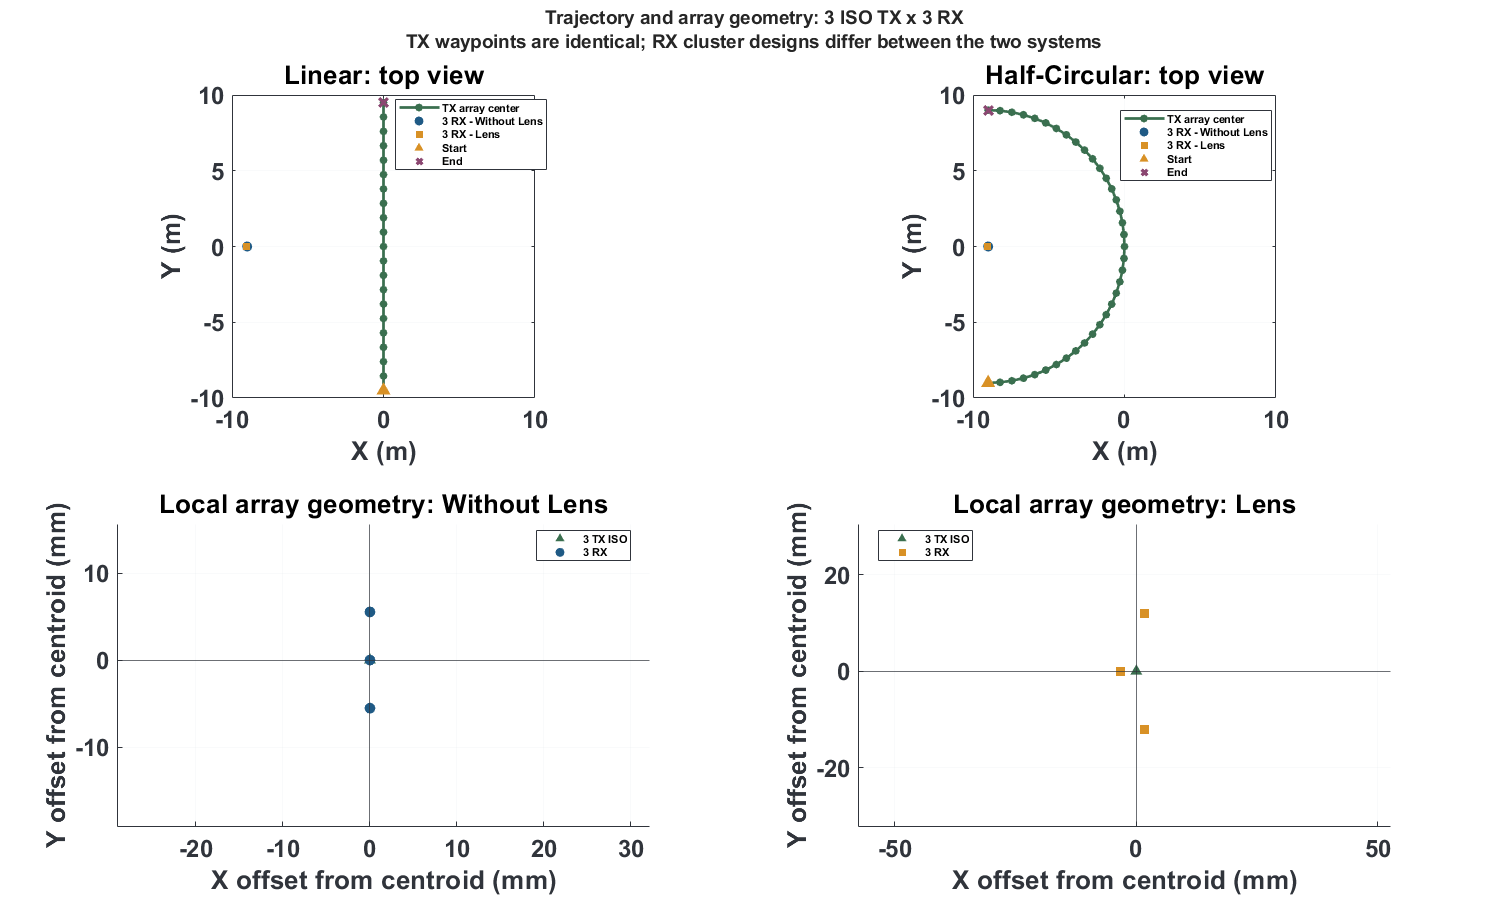
\includegraphics[width=\linewidth]{Images/Analisis_v4_ISO_TX_Lens_vs_WithoutLens_Linear_HalfCircular_3x3/figures_matlab/01_geometry_and_arrays_matlab.png}
    \caption{Paired TX trajectories and local array geometry for the comparison with three isotropic TX elements. The linear and half-circular waypoint sequences are identical for the two RX designs, but the baseline uses a linear RX array, whereas the lens-assisted configuration uses a compact focal-arc arrangement with angle-specific patterns.}
    \label{fig:iso3x3-trajectory-geometry}
\end{figure}
\clearpage

\subsection{Evaluation Metrics and Aggregation}

For each active RX branch, the contributions from the three isotropic TX elements are combined noncoherently at the power level in the link budget. If $H_i(f_k)$ is the channel response of TX element $i$ at frequency $f_k$, the received power, SNR, and equivalent-SISO Shannon capacity are
\begin{equation}
    \begin{aligned}
        P_\mathrm{RX}(f_k)&=P_\mathrm{TX}\sum_{i=1}^{3}|H_i(f_k)|^2,
        &\gamma(f_k)&=\frac{P_\mathrm{RX}(f_k)}{kTB\,10^{\mathrm{NF}/10}},\\
        C_\mathrm{link}&=\frac{1}{N_f}\sum_{k=1}^{N_f}\log_2\!\left(1+\gamma(f_k)\right).
    \end{aligned}
    \label{eq:iso3x3-link-capacity}
\end{equation}
This link-budget capacity represents the aggregate contribution of three simultaneously active TX elements to one active RX branch under the power-summing assumption. It is distinct from the constructed $3\times3$ MIMO capacity described below. In the trajectory workflow, $H_i(f_k)$ in Equation~\ref{eq:iso3x3-link-capacity} is taken from the first mobility time sample at the corresponding waypoint. Thus, $C_\mathrm{link}$ is a frequency-averaged snapshot capacity rather than an average over all 16 mobility samples.

At every waypoint $w$, the three sequential $3\times1$ RX simulations are stacked to form a constructed channel matrix $\mathbf{H}_w(f)$. With singular values $\sigma_{w,1}(f)\geq\cdots\geq\sigma_{w,3}(f)$, the condition number and effective rank are
\begin{equation}
    \begin{aligned}
        \kappa_w(f)&=\frac{\sigma_{w,1}(f)}{\sigma_{w,3}(f)},\\
        p_{w,i}(f)&=\frac{\sigma_{w,i}^2(f)}
        {\sum_{j=1}^{3}\sigma_{w,j}^2(f)},\\
        r_{\mathrm{eff},w}(f)&=\exp\!\left[-\sum_{i=1}^{3}
        p_{w,i}(f)\ln p_{w,i}(f)\right].
    \end{aligned}
    \label{eq:mc3x3-condrank}
\end{equation}

The condition number and effective rank in Equation~\ref{eq:mc3x3-condrank} are evaluated separately in every frequency bin. For a static snapshot and for each trajectory waypoint, the reported scalar condition number and effective rank are the medians over frequency. The aggregate trajectory values reported later are, in turn, medians of these waypoint-level summaries.

Before the fixed-SNR capacity is evaluated, the source notebooks normalize each constructed waypoint channel tensor to unit mean squared coefficient magnitude across RX branches, TX elements, and frequency. For $N_R=N_T=3$ and $N_f$ frequency bins, the normalization is
\begin{equation}
    a_w=
    \sqrt{\frac{1}{N_R N_T N_f}
    \sum_{k=1}^{N_f}\left\lVert\mathbf{H}_w(f_k)\right\rVert_{\mathrm{F}}^2},
    \qquad
    \overline{\mathbf{H}}_w(f_k)=\frac{\mathbf{H}_w(f_k)}{a_w}.
    \label{eq:mc-unit-rms-normalization}
\end{equation}
This convention gives
$\left(N_R N_T N_f\right)^{-1}\sum_k\left\lVert\overline{\mathbf{H}}_w(f_k)\right\rVert_{\mathrm{F}}^2=1$, or, equivalently, an average total normalized channel energy of $N_R N_T=9$ per frequency bin. It differs from the per-frequency unit-Frobenius normalization in Equation~\ref{eq:mimo_frobenius_normalization}, which forces $\lVert\widetilde{\mathbf{H}}(f)\rVert_{\mathrm{F}}^2=1$ in every frequency bin. The scalar $a_w$ does not change the condition number or effective rank, but it sets the scale of the fixed-SNR capacity.

Let $\overline{\sigma}_{w,i}(f_k)$ denote the singular values of $\overline{\mathbf{H}}_w(f_k)$. The ideal equal-power capacity used by the trajectory workflow is
\begin{equation}
    C_{\mathrm{MIMO},w}(\rho)=\frac{1}{N_f}\sum_{k=1}^{N_f}
    \sum_{i=1}^{3}\log_2\!\left(1+\frac{\rho}{N_T}
    \overline{\sigma}_{w,i}^2(f_k)\right),
    \qquad N_T=3,
    \label{eq:mc3x3-mimocapacity}
\end{equation}
with the normalized reference SNR set to $\rho=10$ for the reported 10~dB results. Equation~\ref{eq:mc3x3-mimocapacity} is a frequency average, not an ergodic expectation over independent channel realizations. Because Equation~\ref{eq:mc-unit-rms-normalization} removes the common waypoint channel-amplitude scale, this metric diagnoses spatial and frequency-selective channel structure rather than absolute link-budget performance; it is therefore not directly comparable with $C_\mathrm{link}$ in Equation~\ref{eq:iso3x3-link-capacity}. A smaller condition number and a larger effective rank are favorable. Because the three RX channels are simulated sequentially rather than as simultaneous physical receiver ports, these quantities diagnose spatial structure and diversity potential rather than directly realizable multiport capacity.

The static per-branch plots use a separate normalized single-RX metric. For the channel vector $\mathbf{h}_r(f_k)\in\mathbb{C}^{N_T}$ of RX branch $r$, the source workflow defines
\begin{equation}
    b_r=\sqrt{\frac{1}{N_T N_f}\sum_{k=1}^{N_f}
    \left\lVert\mathbf{h}_r(f_k)\right\rVert_2^2},
    \qquad
    C_{\mathrm{RX},r}(\rho)=\frac{1}{N_f}\sum_{k=1}^{N_f}
    \log_2\!\left(1+\frac{\rho}{N_T}
    \left\lVert\frac{\mathbf{h}_r(f_k)}{b_r}\right\rVert_2^2\right).
    \label{eq:static-normalized-rx-capacity}
\end{equation}
This metric also uses $\rho=10$ for the 10~dB result and removes the absolute channel-amplitude scale. It should not be confused with the link-budget capacity in Equation~\ref{eq:iso3x3-link-capacity}.

Spatial decorrelation is evaluated separately for the center TX element (zero-based index~1) across the three RX responses. Let $h_i[n]$ and $h_j[n]$ be complex channel-frequency-response samples for RX branches $i$ and $j$. Their normalized complex channel coherence, termed correlation in the source workflow, and the corresponding decorrelation are
\begin{equation}
    \rho_{ij}=\frac{\sum_n h_i[n]h_j^*[n]}
    {\sqrt{\left(\sum_n|h_i[n]|^2\right)\left(\sum_n|h_j[n]|^2\right)}},
    \qquad D_{ij}=1-|\rho_{ij}|.
    \label{eq:iso3x3-spatial-correlation}
\end{equation}
No sample-mean subtraction is applied in Equation~\ref{eq:iso3x3-spatial-correlation}; thus, $\rho_{ij}$ is a normalized complex inner product rather than a Pearson correlation coefficient. Two aggregation scopes are retained. The global-pooled value applies Equation~\ref{eq:iso3x3-spatial-correlation} after concatenating all waypoint, time, and frequency samples. The robust estimator evaluates the correlation across the 401 frequency bins in every waypoint--time block and then takes the median for each RX pair,
\begin{equation}
    D_{ij}^{\mathrm{med}}=1-\operatorname{median}_{w,t}\!\left|\rho_{ij}^{(w,t)}\right|.
    \label{eq:iso3x3-median-decorrelation}
\end{equation}
The reported scalar values are means over the unique RX pairs. The along-path pooled curves instead pool time and frequency samples separately within each waypoint, whereas the along-path median-based curves take the median across time blocks at each waypoint. These summaries have different weighting and must not be treated as interchangeable. The unnormalized difference power, $Q_{ij}^{\mathrm{raw}}=N_s^{-1}\sum_n|h_i[n]-h_j[n]|^2$, where $N_s$ is the number of samples, is also retained to show absolute channel-power differences. However, it cannot by itself establish channel independence.

\subsection{Static Snapshot Characterization}

The static snapshot in Figure~\ref{fig:iso3x3-static-rx} illustrates the main design contrast. The without-lens combined gain is almost invariant across the three RX branches, ranging only from $-79.84$ to $-79.75$~dB. The angle-specific lens branches span from $-76.18$ to $-72.98$~dB and are stronger at all three ordinal indices in this snapshot. This range confirms angular selectivity, but it does not imply that all lens branches retain the same advantage as the TX moves. The normalized per-branch capacities from Equation~\ref{eq:static-normalized-rx-capacity} remain close to 3.4~bit/s/Hz for both designs because this snapshot comparison removes the absolute channel-amplitude scale.

\begin{figure}[htbp]
    \centering
    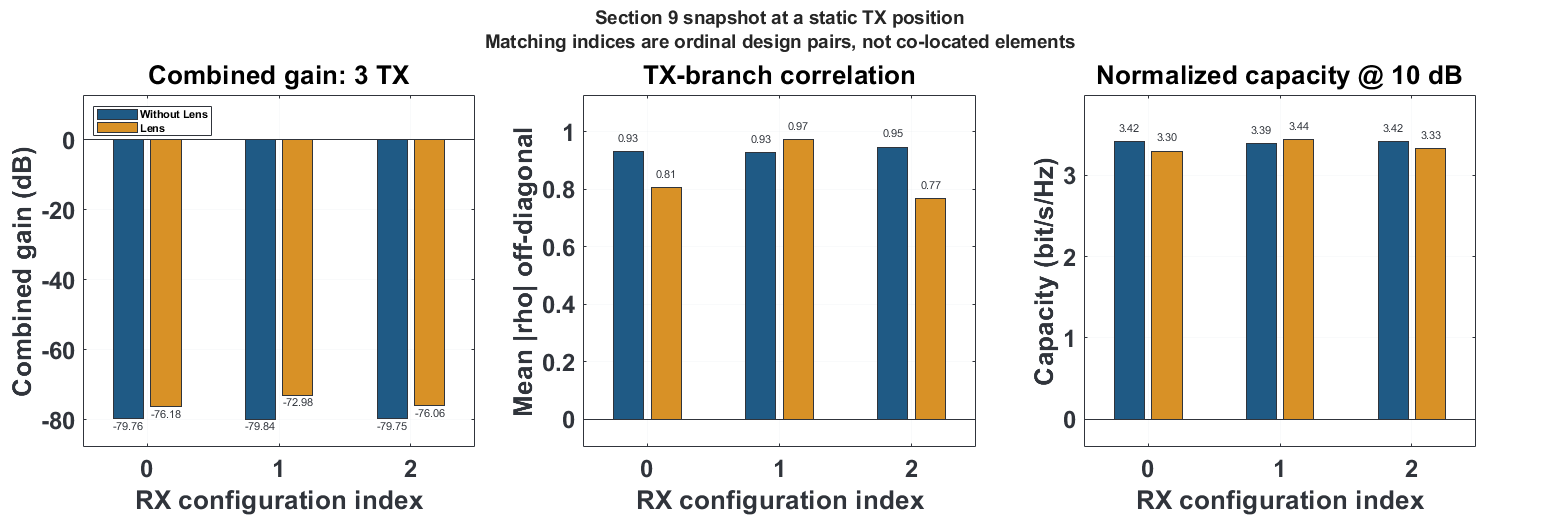
\includegraphics[width=\linewidth]{Images/Analisis_v4_ISO_TX_Lens_vs_WithoutLens_Linear_HalfCircular_3x3/figures_matlab/02_static_rx_scenario_comparison_matlab.png}
    \caption{Static comparison of combined gain, TX-branch correlation, and normalized capacity for the three RX design cases. Matching indices are ordinal design pairs rather than co-located elements.}
    \label{fig:iso3x3-static-rx}
\end{figure}

The constructed static matrix in Figure~\ref{fig:iso3x3-static-mimo} gives a mixed result. With the lens, the snapshot condition number increases from 23.9 to 28.7~dB, while the effective rank rises from 1.42 to 1.60 and the normalized capacity at 10~dB rises from 6.81 to 7.24~bit/s/Hz. The mean magnitude of the off-diagonal RX correlation decreases from 0.7927 to 0.5636. Consequently, the larger condition number does not preclude improvements in the other normalized snapshot metrics; the singular-value distribution, correlation, and capacity must be considered together.

\begin{figure}[htbp]
    \centering
    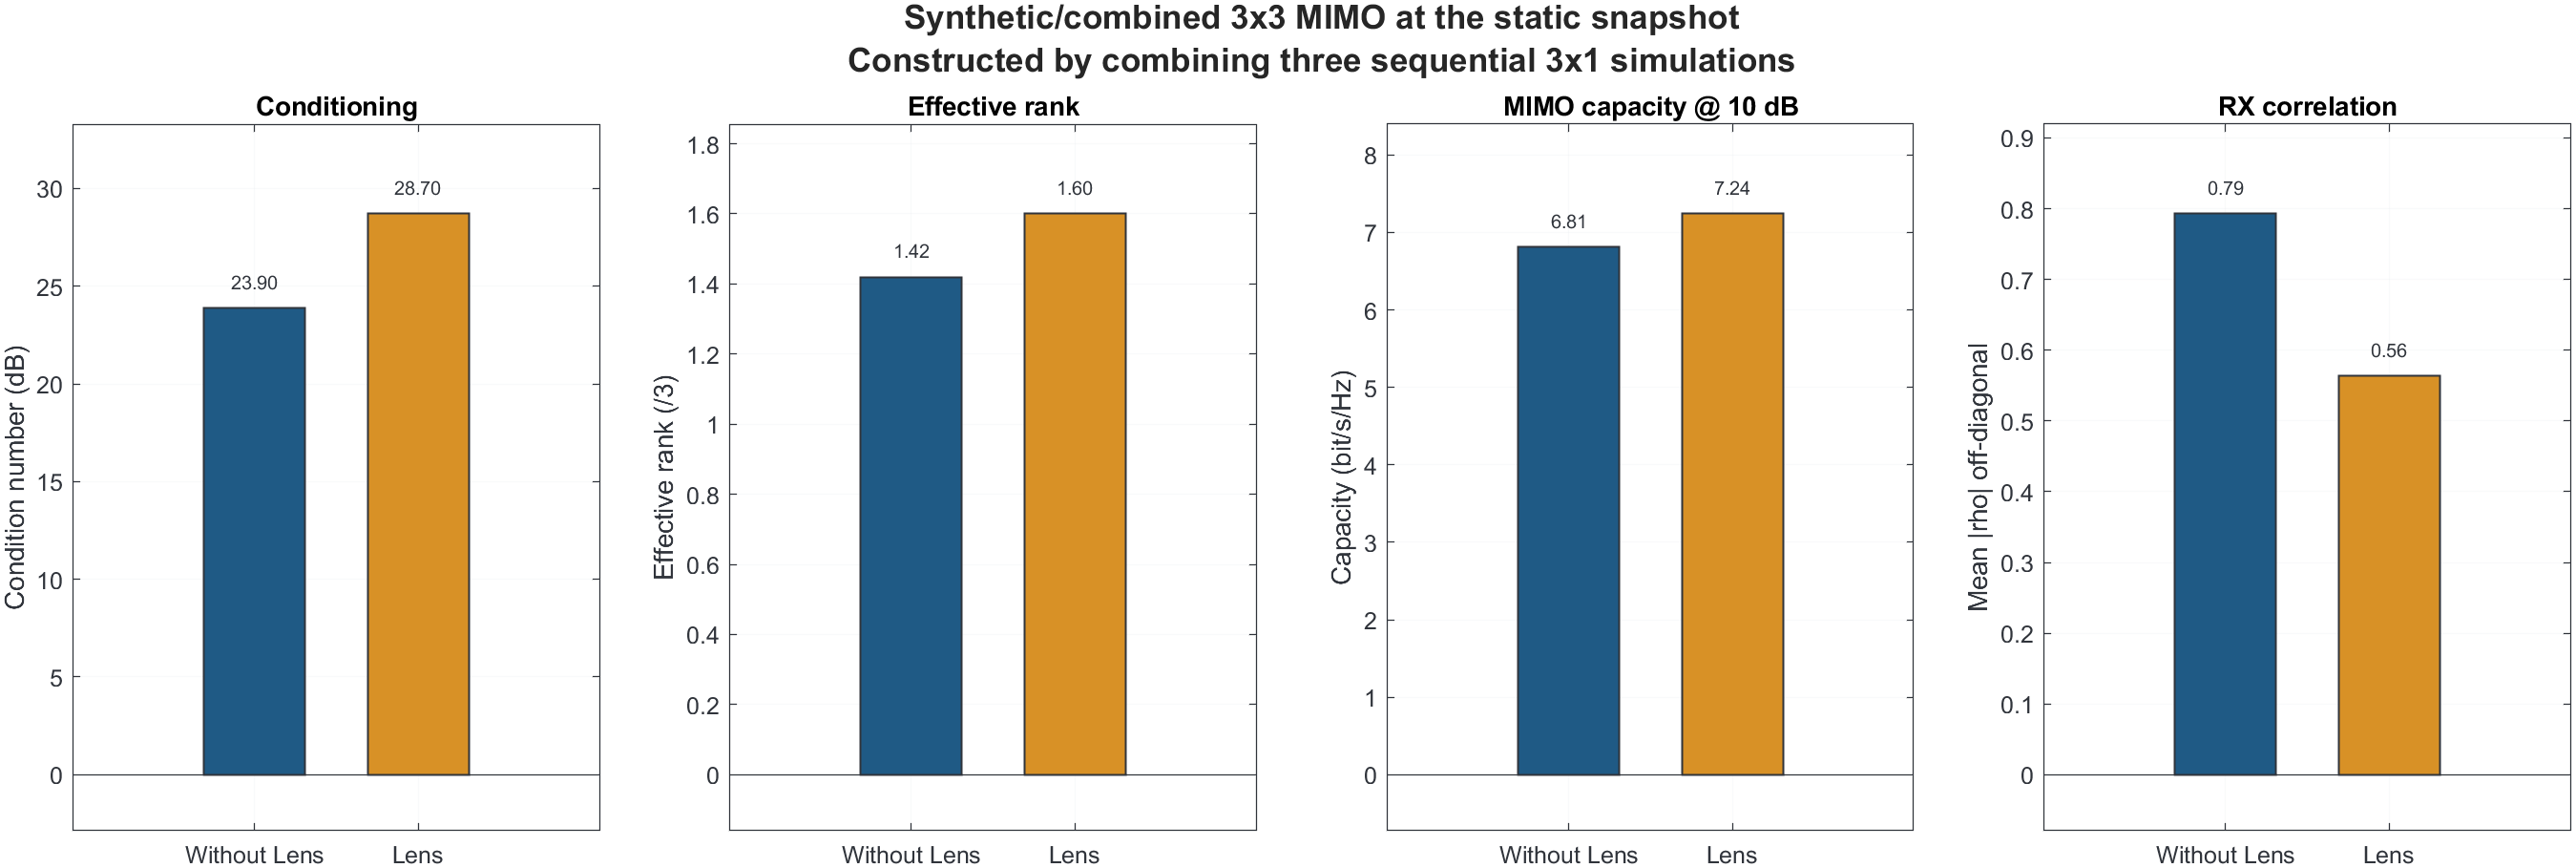
\includegraphics[width=\linewidth]{Images/Analisis_v4_ISO_TX_Lens_vs_WithoutLens_Linear_HalfCircular_3x3/figures_matlab/03_static_mimo_comparison_matlab.png}
    \caption{Constructed $3\times3$ MIMO metrics at the static snapshot. The matrix combines three sequential $3\times1$ RX simulations and is used as a channel-structure diagnostic.}
    \label{fig:iso3x3-static-mimo}
\end{figure}

\subsection{Aggregate and Along-Trajectory Link Performance}

Table~\ref{tab:iso3x3-aggregate-results} and Figure~\ref{fig:iso3x3-aggregate} summarize the main trajectory results. Medians are computed from the complete waypoint--RX population for each configuration. For both paths, the equal-weight ensemble favors the without-lens baseline in channel magnitude and link capacity. On the linear path, the lens decreases median channel magnitude by 7.01~dB and link capacity by 1.84~bit/s/Hz, or 34.01\%. On the half-circular path, the corresponding decreases are 6.40~dB and 1.55~bit/s/Hz, or 30.51\%.

\begin{table}[htbp]
    \centering
    \caption{Aggregate link, constructed-MIMO, and spatial-decorrelation metrics for the paired trajectories. Both capacity columns are in bit/s/Hz. The channel-magnitude summary uses all 16 mobility samples, whereas the link and constructed-MIMO metrics use the first sample at each waypoint. $D_\mathrm{global}$ pools all waypoint, mobility-time, and frequency samples; $D_\mathrm{med}$ is the block-median decorrelation. Both decorrelation values are averaged over unique RX pairs.}
    \label{tab:iso3x3-aggregate-results}
    \scriptsize
    \renewcommand{\arraystretch}{1.15}
    \begin{tabularx}{\linewidth}{@{}>{\raggedright\arraybackslash}p{0.13\linewidth} >{\raggedright\arraybackslash}p{0.14\linewidth} *{7}{>{\centering\arraybackslash}X}@{}}
        \toprule
        \textbf{Path} & \textbf{RX design} & \textbf{$|H|_\mathrm{med}$ (dB)} & \textbf{$C_\mathrm{link}$} & \textbf{$\kappa_\mathrm{med}$ (dB)} & \textbf{$r_\mathrm{eff,med}$} & \textbf{$C_\mathrm{MIMO}$} & \textbf{$D_\mathrm{global}$} & \textbf{$D_\mathrm{med}$} \\
        \midrule
        Linear & Without lens & $-79.74$ & $5.41$ & $25.01$ & $1.202$ & $6.12$ & $0.9784$ & $0.0909$ \\
        Linear & Lens & $-86.75$ & $3.57$ & $25.55$ & $1.154$ & $5.85$ & $0.9807$ & $0.5308$ \\
        Half-circular & Without lens & $-80.89$ & $5.08$ & $25.58$ & $1.348$ & $6.71$ & $0.9744$ & $0.0638$ \\
        Half-circular & Lens & $-87.29$ & $3.53$ & $21.56$ & $1.305$ & $6.58$ & $0.9872$ & $0.5518$ \\
        \bottomrule
    \end{tabularx}
\end{table}

\clearpage
\begin{figure}[p]
    \centering
    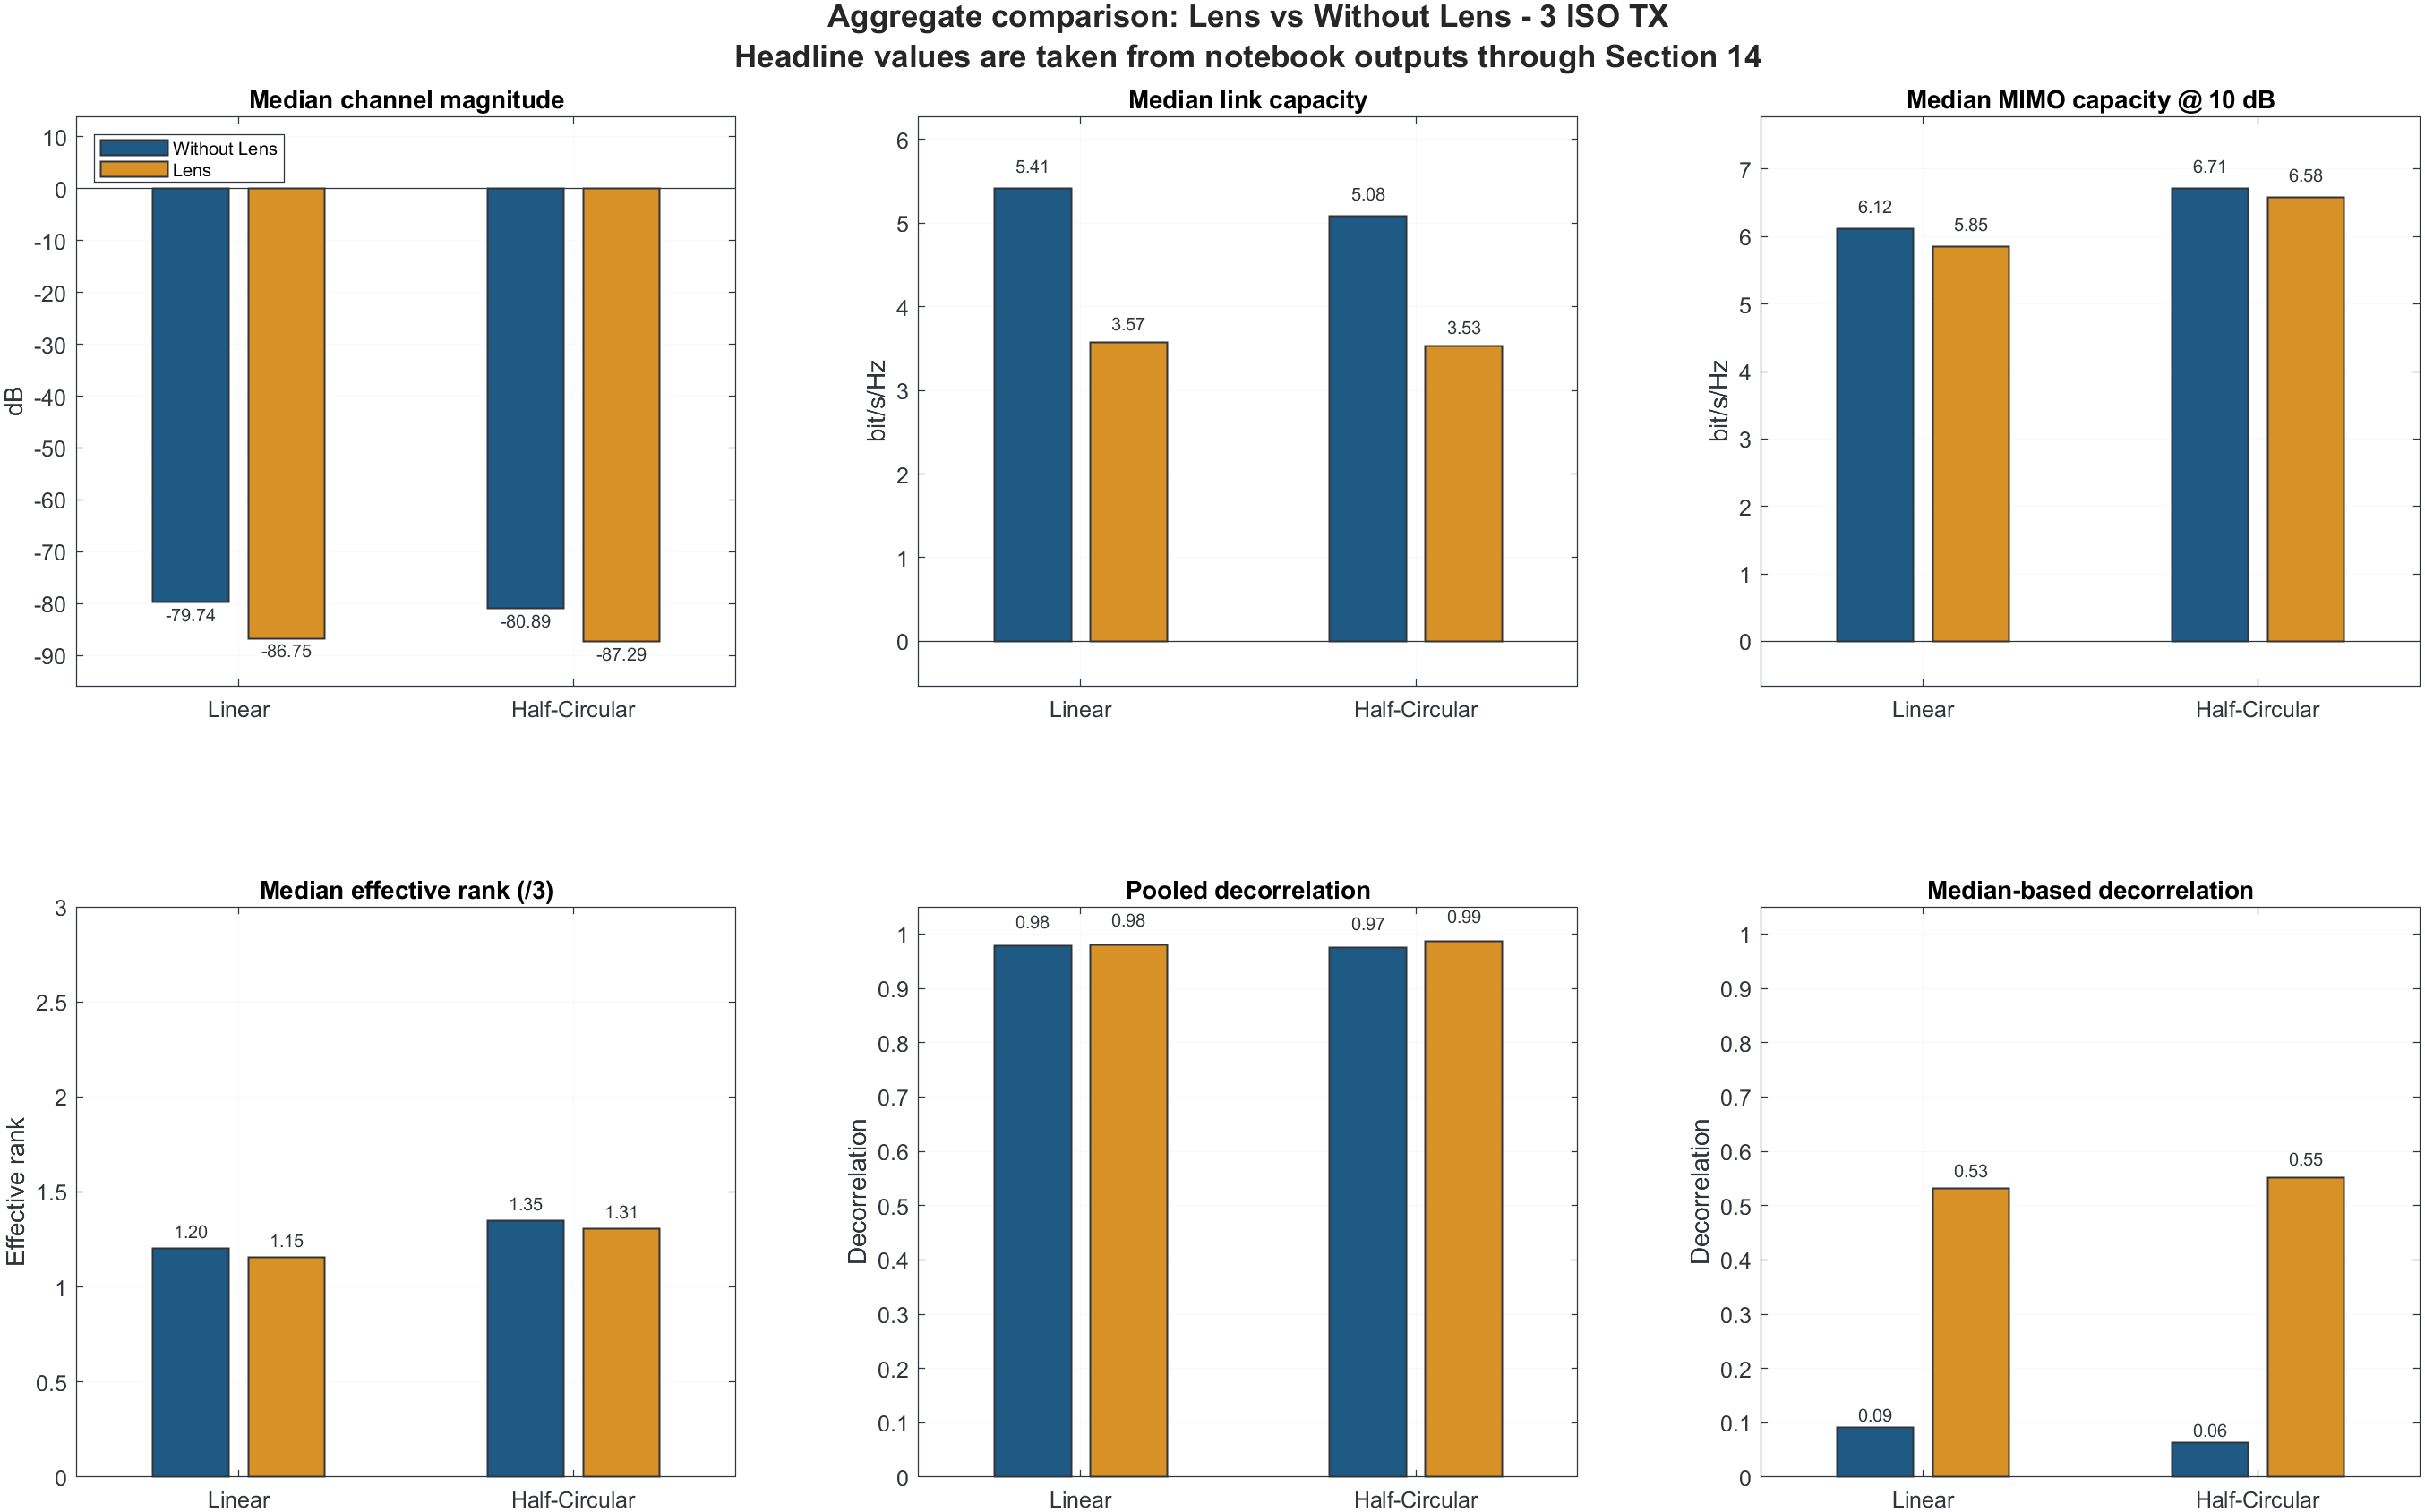
\includegraphics[width=\linewidth]{Images/Analisis_v4_ISO_TX_Lens_vs_WithoutLens_Linear_HalfCircular_3x3/figures_matlab/08_aggregate_comparison_matlab.png}
    \caption{Aggregate comparison of the lens-assisted and without-lens RX designs for three isotropic TX elements. Channel magnitude and link capacity are medians over waypoint--RX observations, although they use all mobility samples and the first sample, respectively. MIMO metrics use the first-sample constructed $3\times3$ channel; spatial decorrelation uses all mobility samples and is reported at both global-pooled and block-median scopes.}
    \label{fig:iso3x3-aggregate}
\end{figure}
\clearpage

Figure~\ref{fig:iso3x3-link-trajectory} shows that the mean without-lens capacity exceeds the mean lens-assisted capacity at all 21 linear-path waypoints and at 28 of the 37 half-circular waypoints. Along some portions of the half-circular path, an aligned lens branch raises the three-branch mean above the baseline. The shaded lens region is the minimum-to-maximum range across the three RX cases, not a confidence interval; its width shows that individual angle-specific branches can be much stronger or weaker than the ensemble mean. All four configurations record 0\% outage at the 1~bit/s/Hz threshold. This threshold is therefore saturated and cannot distinguish reliability; higher thresholds or capacity percentiles are required for an informative outage comparison.

\clearpage
\begin{figure}[p]
    \centering
    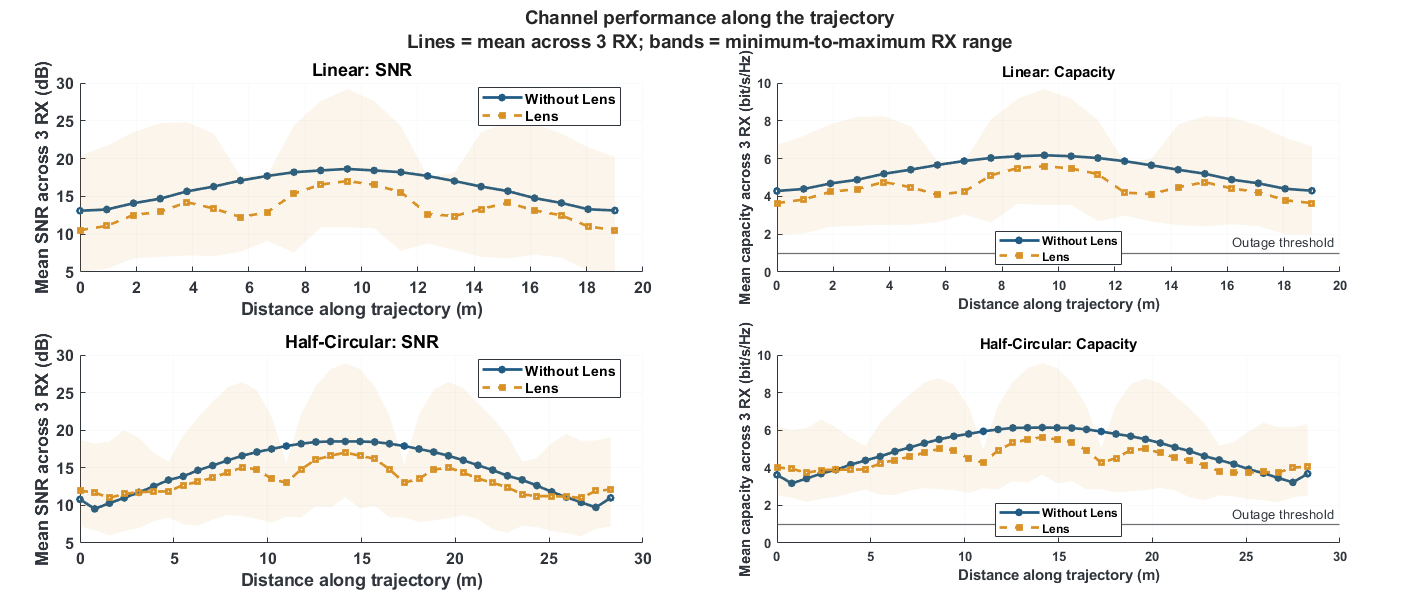
\includegraphics[width=\linewidth]{Images/Analisis_v4_ISO_TX_Lens_vs_WithoutLens_Linear_HalfCircular_3x3/figures_matlab/04_channel_metrics_along_trajectory_matlab.png}
    \caption{Mean SNR and equivalent-SISO link capacity along the linear and half-circular trajectories, evaluated from the first mobility sample at each waypoint. Lines are means across the three RX cases, and the shaded lens bands are the corresponding minimum-to-maximum ranges. The horizontal capacity reference is the 1~bit/s/Hz outage threshold.}
    \label{fig:iso3x3-link-trajectory}
\end{figure}
\clearpage

\subsection{Constructed MIMO Performance Along the Trajectories}

The lens-assisted design produces slightly lower median constructed-MIMO capacity and effective rank on both paths. For the linear trajectory, the median normalized capacity at 10~dB falls from 6.12 to 5.85~bit/s/Hz and the effective rank decreases from 1.202 to 1.154, while the median condition number worsens by 0.55~dB, from 25.01 to 25.55~dB. For the half-circular trajectory, capacity falls from 6.71 to 6.58~bit/s/Hz and effective rank from 1.348 to 1.305, but the condition number improves from 25.58 to 21.56~dB. Thus, the sizeable conditioning improvement on the half-circular path does not translate into a higher median rank or capacity under the present construction.

Figure~\ref{fig:iso3x3-mimo-trajectory} also reveals a pronounced impairment at the geometrically symmetric 9.5~m midpoint of the linear path: the condition number reaches 65.69~dB without the lens and 55.09~dB with the lens, while the corresponding capacities fall to 5.14 and 5.19~bit/s/Hz. The half-circular trajectory avoids such a severe common midpoint conditioning peak and yields a higher median effective rank and MIMO capacity for both designs. This between-path difference is descriptive, however, because path shape, location, distance distribution, and waypoint count vary together.

\clearpage
\begin{figure}[p]
    \centering
    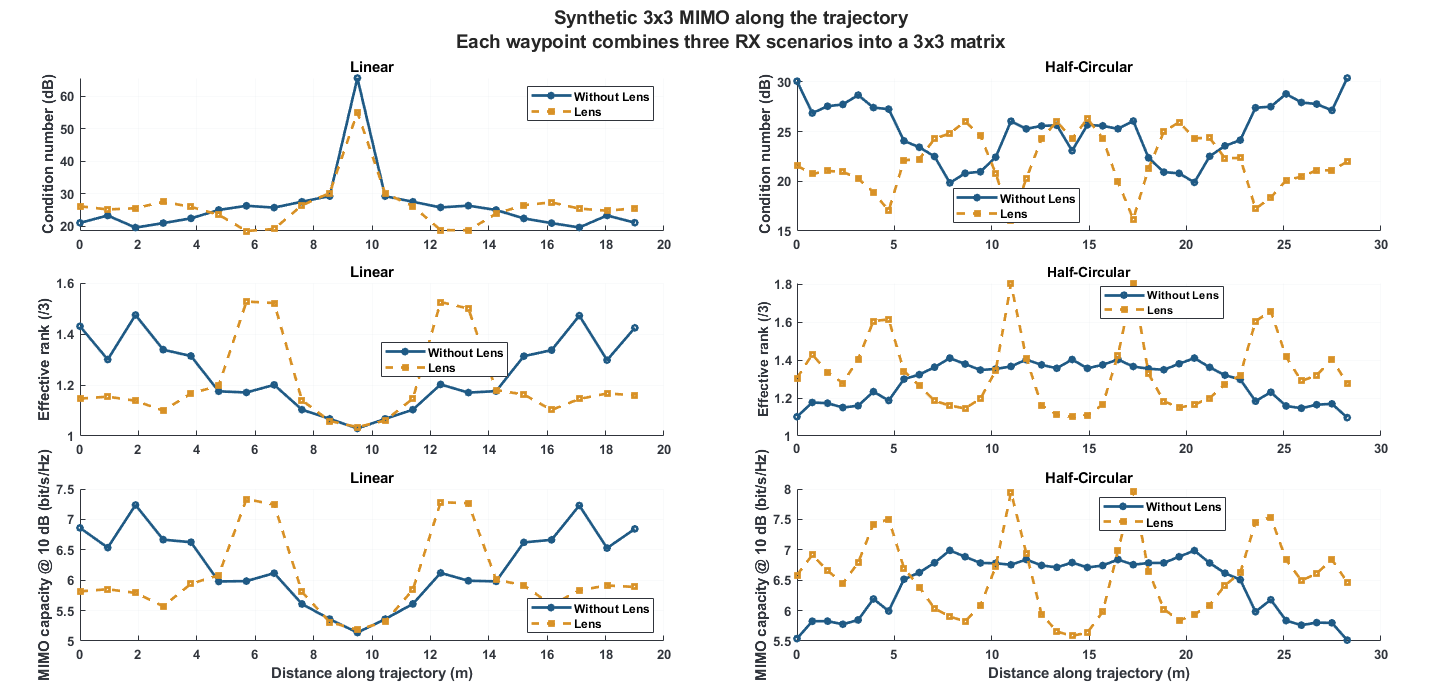
\includegraphics[width=\linewidth]{Images/Analisis_v4_ISO_TX_Lens_vs_WithoutLens_Linear_HalfCircular_3x3/figures_matlab/05_trajectory_mimo_metrics_matlab.png}
    \caption{Condition number, effective rank, and ideal normalized capacity at 10~dB for the constructed $3\times3$ channel along the two trajectories. The linear midpoint produces a pronounced conditioning peak in both configurations.}
    \label{fig:iso3x3-mimo-trajectory}
\end{figure}
\clearpage

\subsection{Spatial Decorrelation}

Both spatial estimators favor the lens, although the magnitude of the effect depends strongly on aggregation scope. When all realizations are concatenated before normalization, global pooled decorrelation increases only slightly, from 0.9784 to 0.9807 on the linear path and from 0.9744 to 0.9872 on the half-circular path. By contrast, block-median decorrelation increases from 0.0909 to 0.5308 on the linear path and from 0.0638 to 0.5518 on the half-circular path. The waypoint-level curves in Figure~\ref{fig:iso3x3-decorrelation} likewise favor the lens: mean waypoint-level pooled decorrelation is 0.5502 with the lens versus 0.1112 without it on the linear path and 0.5275 versus 0.0704 on the half-circular path.

The global statistic measures the coherence of the complete concatenated response, whereas the block-median and waypoint-level summaries give more comparable weight to local conditions. Their different effect sizes therefore reflect different weighting rather than a contradiction. In addition, these metrics use only the center TX element, so they should not be equated with the full constructed $3\times3$ singular-value metrics.

\begin{figure}[htbp]
    \centering
    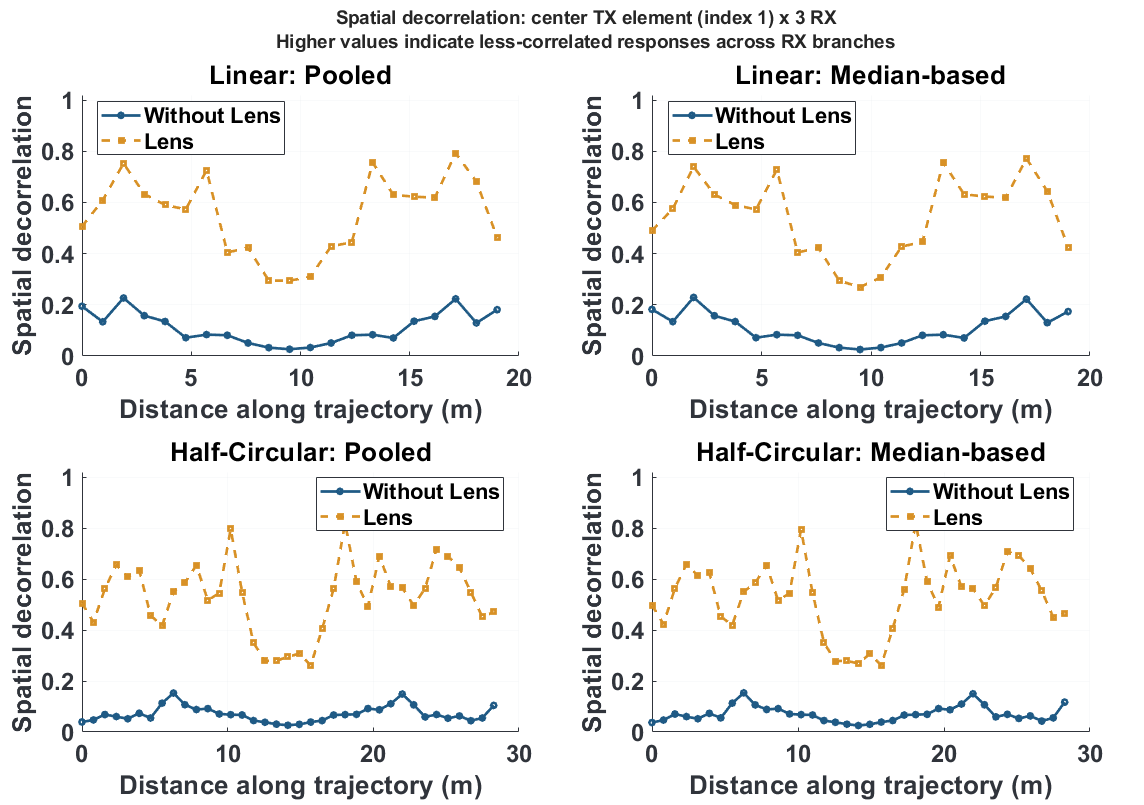
\includegraphics[width=\linewidth]{Images/Analisis_v4_ISO_TX_Lens_vs_WithoutLens_Linear_HalfCircular_3x3/figures_matlab/06_spatial_decorrelation_comparison_matlab.png}
    \caption{Waypoint-level pooled and median-based spatial decorrelation of the center TX element (zero-based index~1) across three RX branches, using all 16 mobility samples. Higher values indicate less-correlated local RX responses; these curves use a different aggregation scope from the global-pooled values in Table~\ref{tab:iso3x3-aggregate-results}.}
    \label{fig:iso3x3-decorrelation}
\end{figure}

The unnormalized difference power in Figure~\ref{fig:iso3x3-raw-difference} supplies amplitude context. Its ordering reflects both path loss and the RX-pattern gain, as well as the difference between channel responses. A larger value therefore cannot independently be interpreted as better decorrelation or higher multiplexing capacity.

\begin{figure}[htbp]
    \centering
    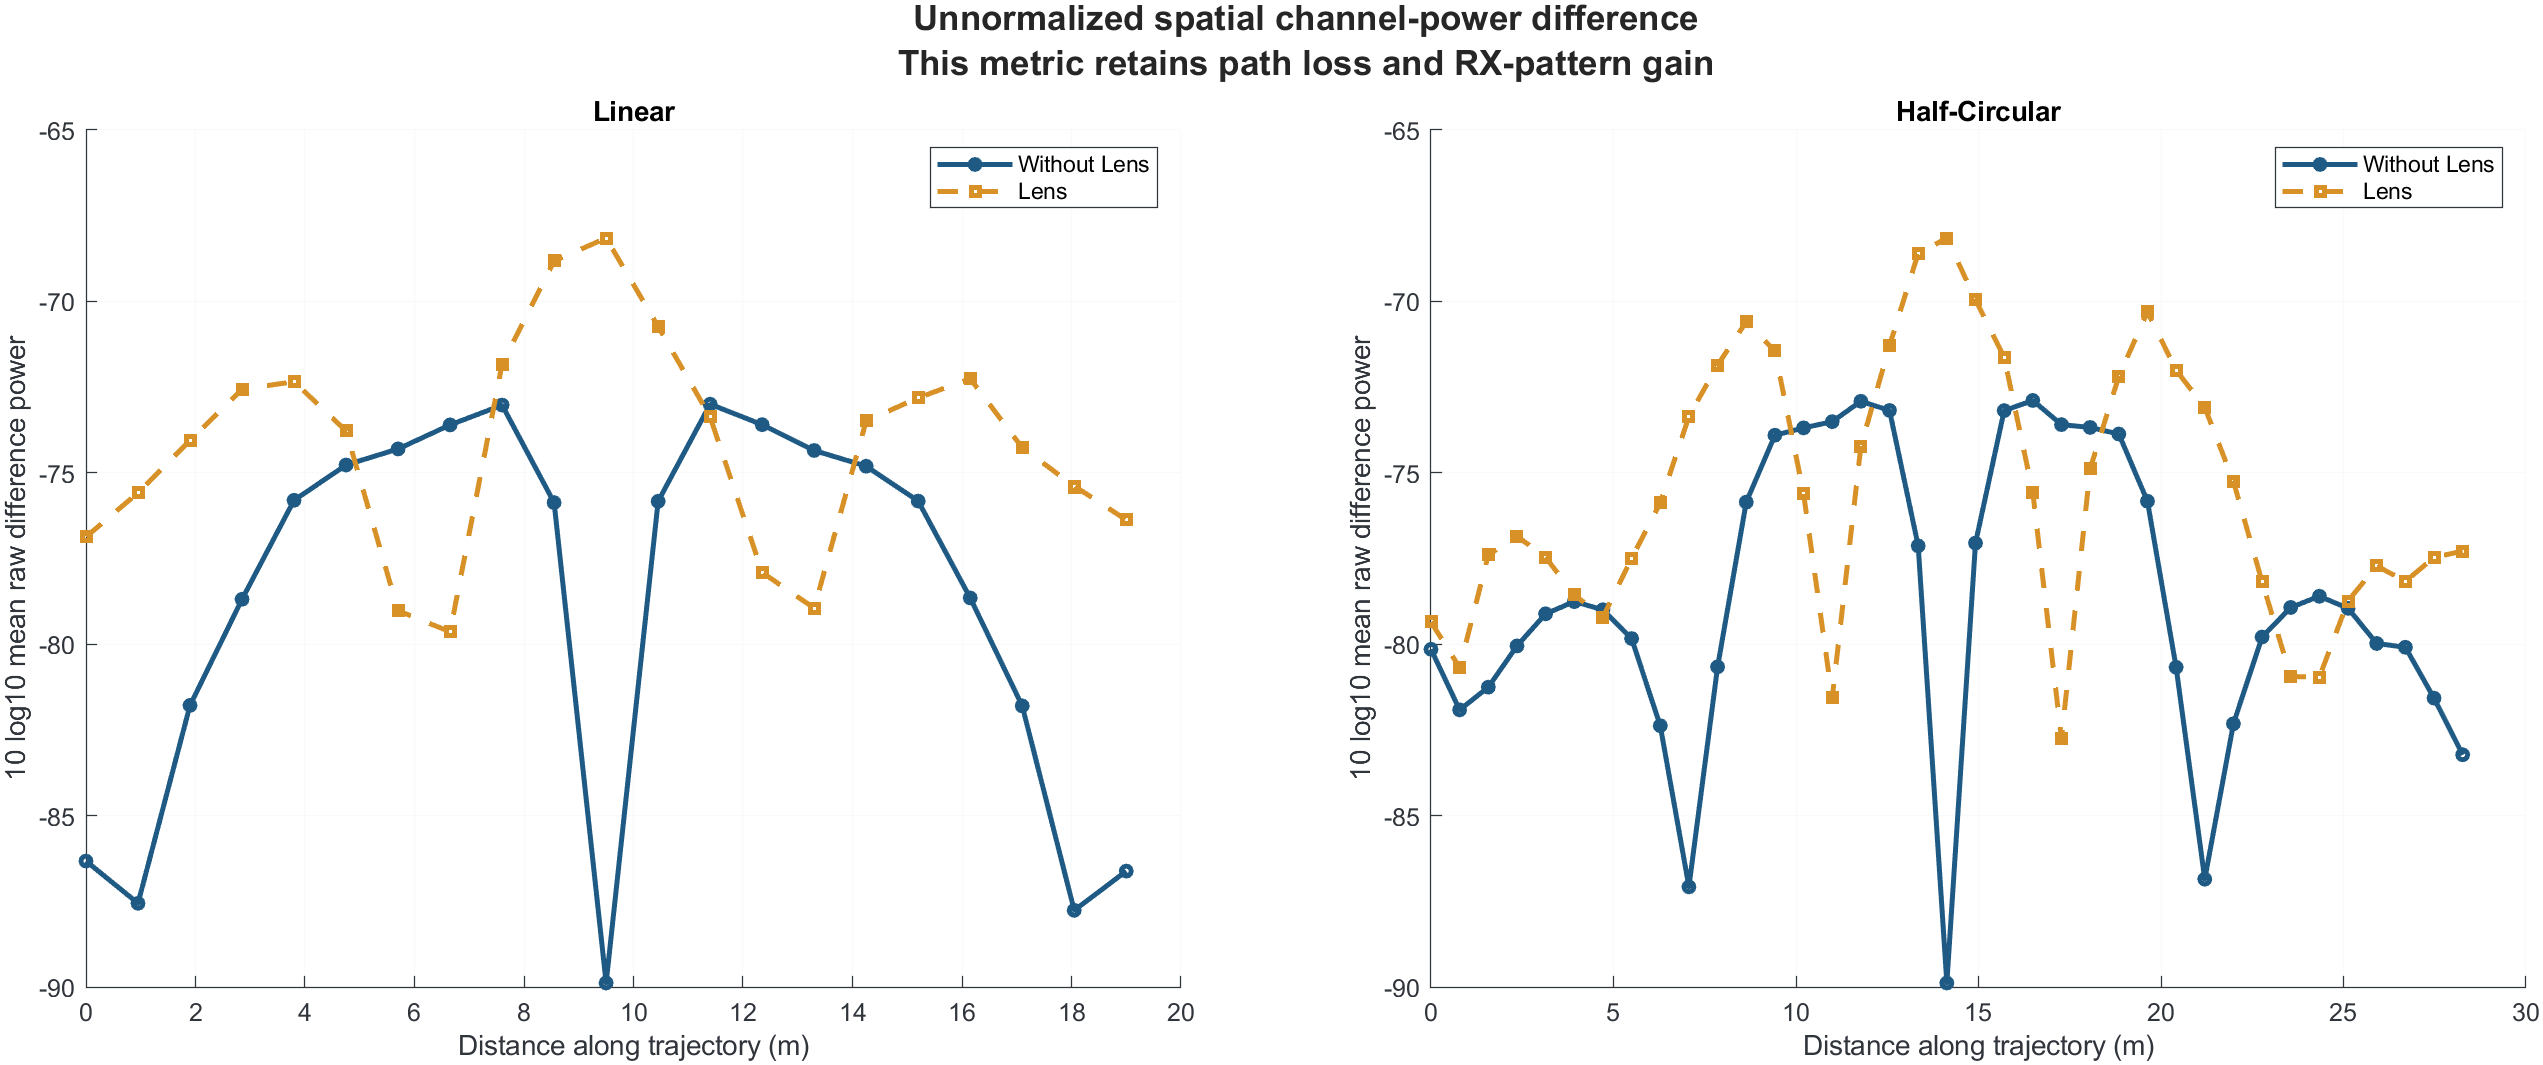
\includegraphics[width=\linewidth]{Images/Analisis_v4_ISO_TX_Lens_vs_WithoutLens_Linear_HalfCircular_3x3/figures_matlab/07_raw_spatial_difference_power_matlab.png}
    \caption{Unnormalized spatial difference power along the linear and half-circular paths. Because the metric retains path loss and RX-pattern gain, it is interpreted only alongside the normalized decorrelation and link-budget metrics.}
    \label{fig:iso3x3-raw-difference}
\end{figure}

\subsection{Discussion and Limitations}

The combined results indicate a trade-off between uniform link performance and angular selectivity. The baseline applies the same patch pattern at three closely spaced positions and therefore gives nearly uniform branch responses. The lens configuration instead samples three directional patterns. Its median within-waypoint link-capacity range is 5.32~bit/s/Hz on the linear path and 4.42~bit/s/Hz on the half-circular path, compared with only 0.01~bit/s/Hz on both paths without the lens. At a given waypoint, one or more aligned beams can therefore be strong while nonaligned beams are weak. Assigning equal statistical weight to all three RX configurations lowers the reported lens median even though the local responses are more differentiated. The present result is specific to reporting all branches without selection and should not be generalized to a receiver that performs beam selection or combining. Such an operating strategy must be evaluated explicitly using a practical selection rule and accounting for switching overhead.

The half-circular path is more favorable to the constructed MIMO metrics for both RX designs because it avoids the severe midpoint conditioning peak of the linear path and samples a broader sequence of relative angles. The available experiment does not isolate trajectory curvature as the cause, since the two paths also differ in position, distance distribution, length, and sample count. Only lens versus without-lens differences within the same trajectory are paired comparisons.

Several limitations constrain the inference. First, each constructed $3\times3$ matrix combines three sequential $3\times1$ RX simulations, so simultaneous multiport reception, mutual coupling, and a common inter-port hardware phase reference are not represented. Second, RX placement and far-field pattern differ together, preventing attribution to the lens material or focal displacement alone. Third, although 16 mobility samples are generated at every waypoint, the reported link-budget SNR and capacity and the constructed-MIMO condition number, effective rank, and capacity use only the first mobility sample; only the time-resolved magnitude and spatial-decorrelation analyses use the complete mobility tensor. The reported capacities therefore do not quantify within-waypoint Doppler variability. Fourth, the results cover one scene and one ray-tracing realization set, without a multi-seed convergence study or confidence intervals. Fifth, 100{,}000 path samples per source were used, whereas the source workflow recommends 1{,}000{,}000 for a final high-accuracy run. Sixth, the along-path SNR and capacity curves were recovered from rounded notebook logs, although the headline medians use the higher-precision stored summaries. Finally, the exported package contains derived tables and figures rather than the complete complex CFR tensor. The capacities are ideal Shannon or fixed-SNR channel metrics and are not predictions of coded throughput.

\subsection{Summary of the Receiver-Configuration Comparison}

For three simultaneous isotropic TX elements and equal statistical weighting of all three RX configurations, the without-lens baseline provides stronger aggregate link performance and slightly higher constructed-MIMO capacity and effective rank on the two evaluated trajectories. Relative to the baseline, the lens reduces median link capacity by 1.84~bit/s/Hz on the linear path and 1.55~bit/s/Hz on the half-circular path, while constructed-MIMO capacity decreases by 0.27 and 0.13~bit/s/Hz, respectively. The lens nevertheless increases both global-pooled and typical-block decorrelation, with the much larger block-median changes confirming stronger local angular differentiation. The half-circular path avoids the pronounced linear-path midpoint conditioning peak and yields higher median effective rank and constructed-MIMO capacity for both designs, but this is a descriptive path comparison. Future work should evaluate practical beam selection and combining, repeat the comparison at co-located RX coordinates, increase the path-sample count, use multiple random seeds, retain the full complex CFR tensor, and adopt informative outage thresholds or capacity percentiles.

\section{Higher-Order MIMO Systems}\label{sec:higher-order-mimo}

This section compares the complete lens-assisted $N\times N$ configurations for $N=3$, $5$, and $9$ using their corresponding Sionna-RT linear-trajectory datasets. In every configuration, $N$ isotropic TX elements radiate simultaneously, and the center of the TX array follows the same 21-waypoint path. The main result is a trade-off: increasing $N$ raises both the link-budget capacity and the fixed-SNR constructed-MIMO capacity, but the median condition number worsens, while the effective rank per dimension and MIMO capacity per dimension decrease.

This trend is a configuration-level scaling result rather than a causal estimate of antenna order alone. The simulations apply 10~dBm to every TX element, keep the inter-element spacing fixed, and assign a different lens-angle grid to each order. Consequently, nominal total TX power, physical aperture, number of RX scenarios, and angular sampling all change with $N$.

\subsection{Simulation Configuration and Order Comparability}

The common environment is a $20\,\text{m}\times20\,\text{m}\times3\,\text{m}$ room at 38~GHz. The channel is sampled over a 400~MHz bandwidth using 401 frequency bins. The linear trajectory runs from $y=-9.5$~m to $y=+9.5$~m at $x=0$ and $z=2$~m, giving 21 waypoints and a total length of 19~m. Motion is evaluated at 1~m/s, with 16 time samples per waypoint at a sampling rate of 1~kHz. As in the receiver-configuration comparison, the channel-magnitude and spatial-decorrelation analyses use all 16 samples in the time-resolved tensor, whereas the link-budget and constructed-MIMO metrics use only the first mobility sample at each waypoint. All configurations use a 7~dB receiver noise figure at 290~K and 100{,}000 path samples per source.

Table~\ref{tab:iso-order-simulation-setup} lists the quantities that change with order. The 0.45~m TX spacing expands the aperture from 0.90 to 3.60~m. Because the power is fixed at 10~dBm per TX, nominal total TX power rises by 4.77~dB from $N=3$ to $N=9$. The RX grids also differ; only the $0^\circ$ lens branch is common to all three configurations. The 63, 105, and 189 observations are waypoint--RX combinations, not independent Monte Carlo drops.

\begin{table}[htbp]
    \centering
    \caption{Order-dependent parameters for the lens-assisted linear-trajectory comparison.}
    \label{tab:iso-order-simulation-setup}
    \footnotesize
    \renewcommand{\arraystretch}{1.15}
    \begin{tabularx}{\linewidth}{@{}>{\centering\arraybackslash}p{0.10\linewidth} >{\centering\arraybackslash}p{0.16\linewidth} >{\raggedright\arraybackslash}X >{\centering\arraybackslash}p{0.17\linewidth} >{\centering\arraybackslash}p{0.16\linewidth}@{}}
        \toprule
        \textbf{Order} & \textbf{TX aperture} & \textbf{RX lens-angle grid} & \textbf{Waypoint--RX observations} & \textbf{Nominal total TX power} \\
        \midrule
        $3\times3$ & 0.90~m & $-45^\circ,0^\circ,+45^\circ$ & 63 & 14.77~dBm \\
        $5\times5$ & 1.80~m & $-60^\circ$ to $+60^\circ$ in $30^\circ$ steps & 105 & 16.99~dBm \\
        $9\times9$ & 3.60~m & $-60^\circ$ to $+60^\circ$ in $15^\circ$ steps & 189 & 19.54~dBm \\
        \bottomrule
    \end{tabularx}
\end{table}

Figure~\ref{fig:iso-order-geometry} shows the common trajectory and the order-dependent TX and RX geometries. The increasingly dense lens grid does not compare the same set of physical RX branches at every order. Accordingly, the aggregate comparisons characterize each complete design, whereas the common $0^\circ$ branch is retained as a narrower sensitivity check.

\begin{figure}[htbp]
    \centering
    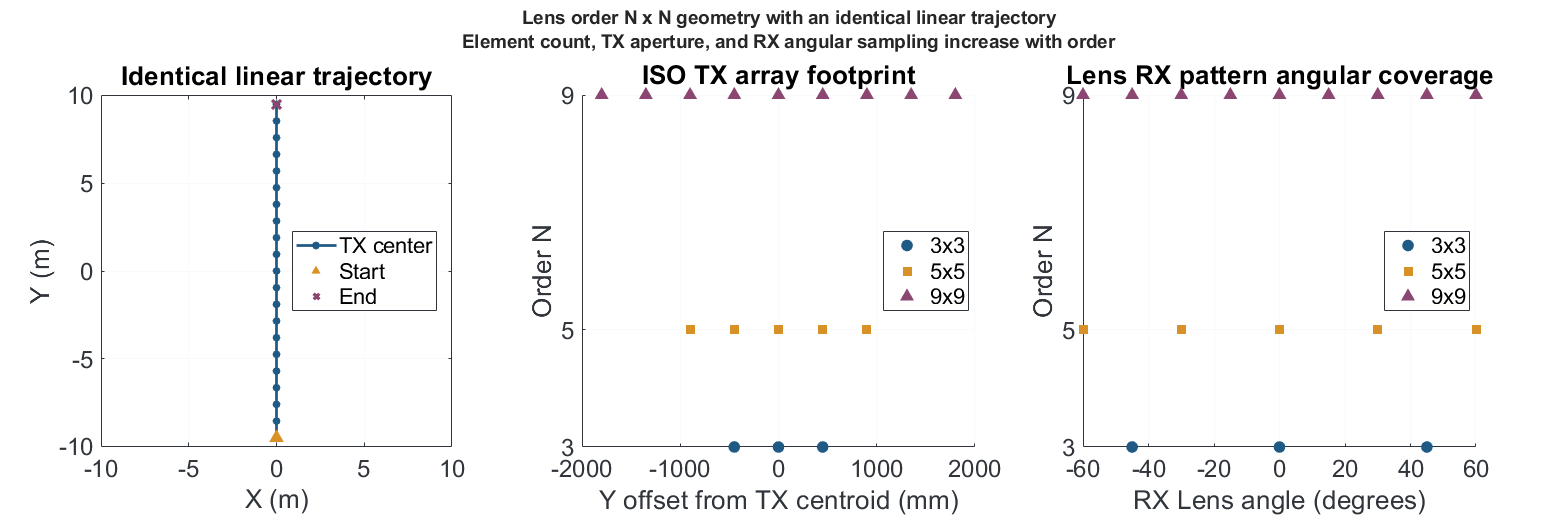
\includegraphics[width=\linewidth]{Images/Analisis_v4_ISO_TX_Lens_Order_3x3_5x5_9x9_Linear/figures_matlab/01_geometry_order_comparison_matlab.png}
    \caption{Common linear TX trajectory and order-dependent TX aperture and RX lens-angle grids for the $3\times3$, $5\times5$, and $9\times9$ configurations.}
    \label{fig:iso-order-geometry}
\end{figure}

\subsection{Metrics and Normalization}

The link-budget capacity follows Equation~\ref{eq:iso3x3-link-capacity}, with the TX summation limit generalized from 3 to $N$. It combines the received power from all simultaneously active TX elements at one active RX branch. The aggregate link statistics pool all waypoint--RX observations within an order. They therefore include both the growing nominal total TX power and the different RX-angle populations.

For the spatial analysis, the $N$ sequential $N\times1$ RX simulations at each waypoint are stacked to construct an $N\times N$ channel matrix. Equations~\ref{eq:mc3x3-condrank}--\ref{eq:mc3x3-mimocapacity} are applied after replacing each upper limit of 3 and $N_T=3$ with $N$. In particular, Equation~\ref{eq:mc-unit-rms-normalization} sets the mean squared magnitude of the $N^2$ channel coefficients, averaged over all 401 frequency bins, to unity separately at every waypoint. Consequently,
\begin{equation}
    \frac{1}{N_f}\sum_{k=1}^{N_f}
    \left\lVert\overline{\mathbf{H}}_w(f_k)\right\rVert_{\mathrm{F}}^2=N^2.
    \label{eq:iso-order-rms-energy}
\end{equation}
The reported condition number is $20\log_{10}\kappa$, and the ideal equal-power MIMO capacity is evaluated at $\rho=10$ with the factor $1/N_T$ in Equation~\ref{eq:mc3x3-mimocapacity}. This normalization holds the average per-coefficient power constant rather than the total normalized channel energy. The constructed capacity can therefore grow naturally as receive and transmit dimensions are added; it should be interpreted together with the per-dimension metrics below. This capacity diagnoses channel structure and dimensional scaling and is distinct from the absolute link-budget capacity. Moreover, the sequentially simulated RX branches do not represent simultaneous physical receiver ports.

Absolute metrics naturally tend to grow when dimensions are added. Two normalized quantities are therefore used to evaluate how efficiently the available dimensions are utilized:
\begin{equation}
    \eta_r(N)=\frac{r_\mathrm{eff}}{N},
    \qquad
    \eta_C(N)=\frac{C_\mathrm{MIMO}(10~\mathrm{dB})}{N}.
    \label{eq:iso-order-normalized-metrics}
\end{equation}
A favorable dimensional-scaling trend increases $C_\mathrm{MIMO}$ without materially reducing $\eta_r$ or $\eta_C$.

Spatial decorrelation follows Equations~\ref{eq:iso3x3-spatial-correlation} and~\ref{eq:iso3x3-median-decorrelation} using the center TX element, corresponding to zero-based indices 1, 2, and 4 for $N=3$, $5$, and $9$, respectively. The global-pooled estimator concatenates all realizations before normalization, whereas the block-median estimator characterizes a typical local block. Figure~\ref{fig:iso-order-decorrelation} uses waypoint-local aggregation, so its curves need not equal the global summary values. The raw difference power remains amplitude-sensitive and is interpreted only as supporting context.

\subsection{Static Snapshot Scaling}

The static RX results in Figure~\ref{fig:iso-order-static-rx} show that the center-branch combined gain improves from $-72.98$~dB for $N=3$ to $-70.71$~dB for $N=5$ and $-69.94$~dB for $N=9$. The normalized per-branch capacity from Equation~\ref{eq:static-normalized-rx-capacity}, generalized to each value of $N$, remains close to 3.4~bit/s/Hz because the static comparison removes the absolute channel-amplitude scale. These values therefore illustrate angular response and normalized channel structure rather than the absolute link-budget advantage of the higher nominal total TX power.

\begin{figure}[htbp]
    \centering
    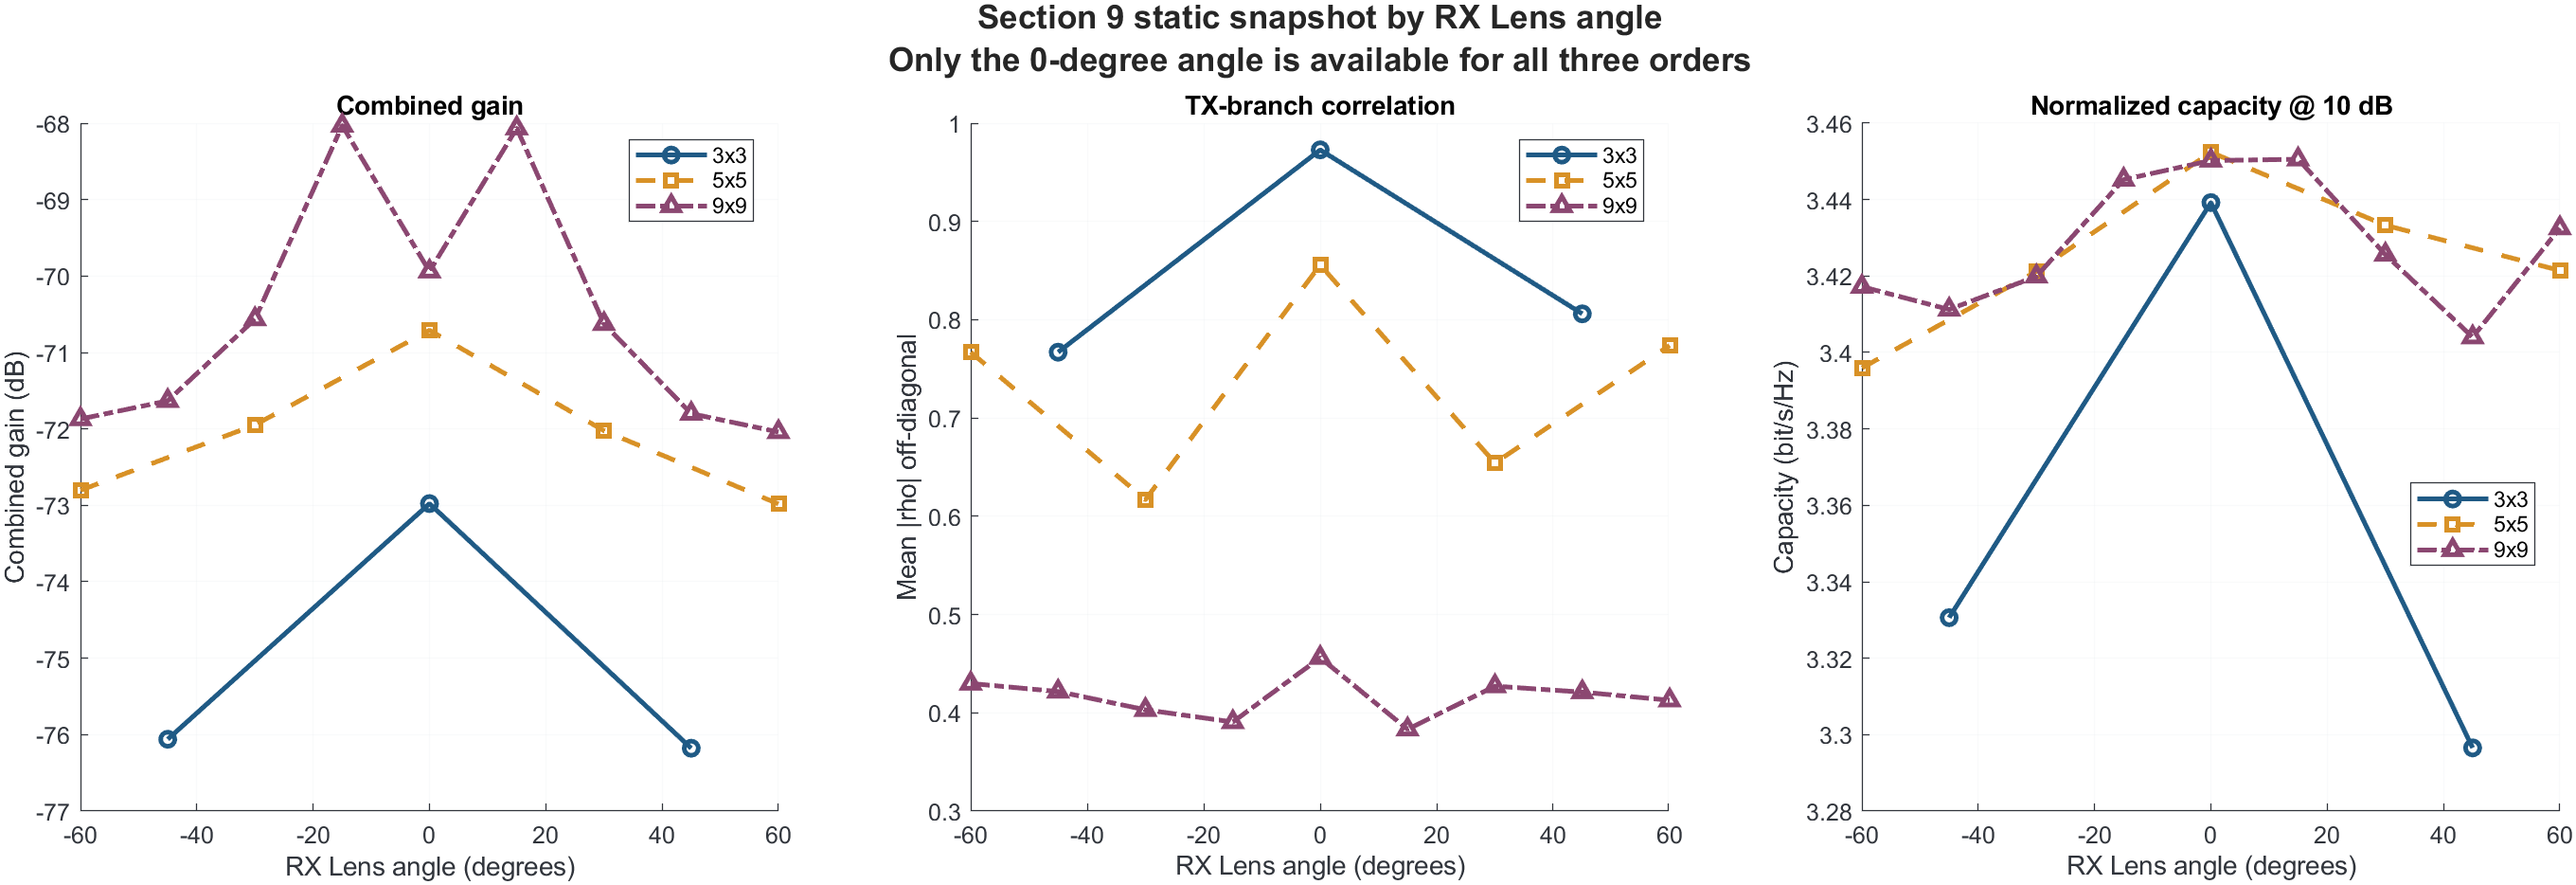
\includegraphics[width=\linewidth]{Images/Analisis_v4_ISO_TX_Lens_Order_3x3_5x5_9x9_Linear/figures_matlab/02_static_rx_by_order_matlab.png}
    \caption{Static combined gain, TX-channel correlation, and normalized per-RX capacity for the three lens-assisted orders. The RX angle grids differ with order.}
    \label{fig:iso-order-static-rx}
\end{figure}

The constructed static matrix does not exhibit a monotonic conditioning trend. As Figure~\ref{fig:iso-order-static-mimo} shows, the condition number is 28.70, 23.40, and 25.10~dB for $N=3$, $5$, and $9$, respectively. The $5\times5$ snapshot also has the largest normalized effective rank (0.666) and capacity per dimension (2.810~bit/s/Hz), compared with 0.533 and 2.413~bit/s/Hz for $N=3$ and 0.569 and 2.653~bit/s/Hz for $N=9$. Meanwhile, mean RX correlation decreases from 0.5636 to 0.2674 as $N$ increases. Thus, the static position suggests favorable angular diversity at higher order, but it cannot represent the complete trajectory.

\begin{figure}[htbp]
    \centering
    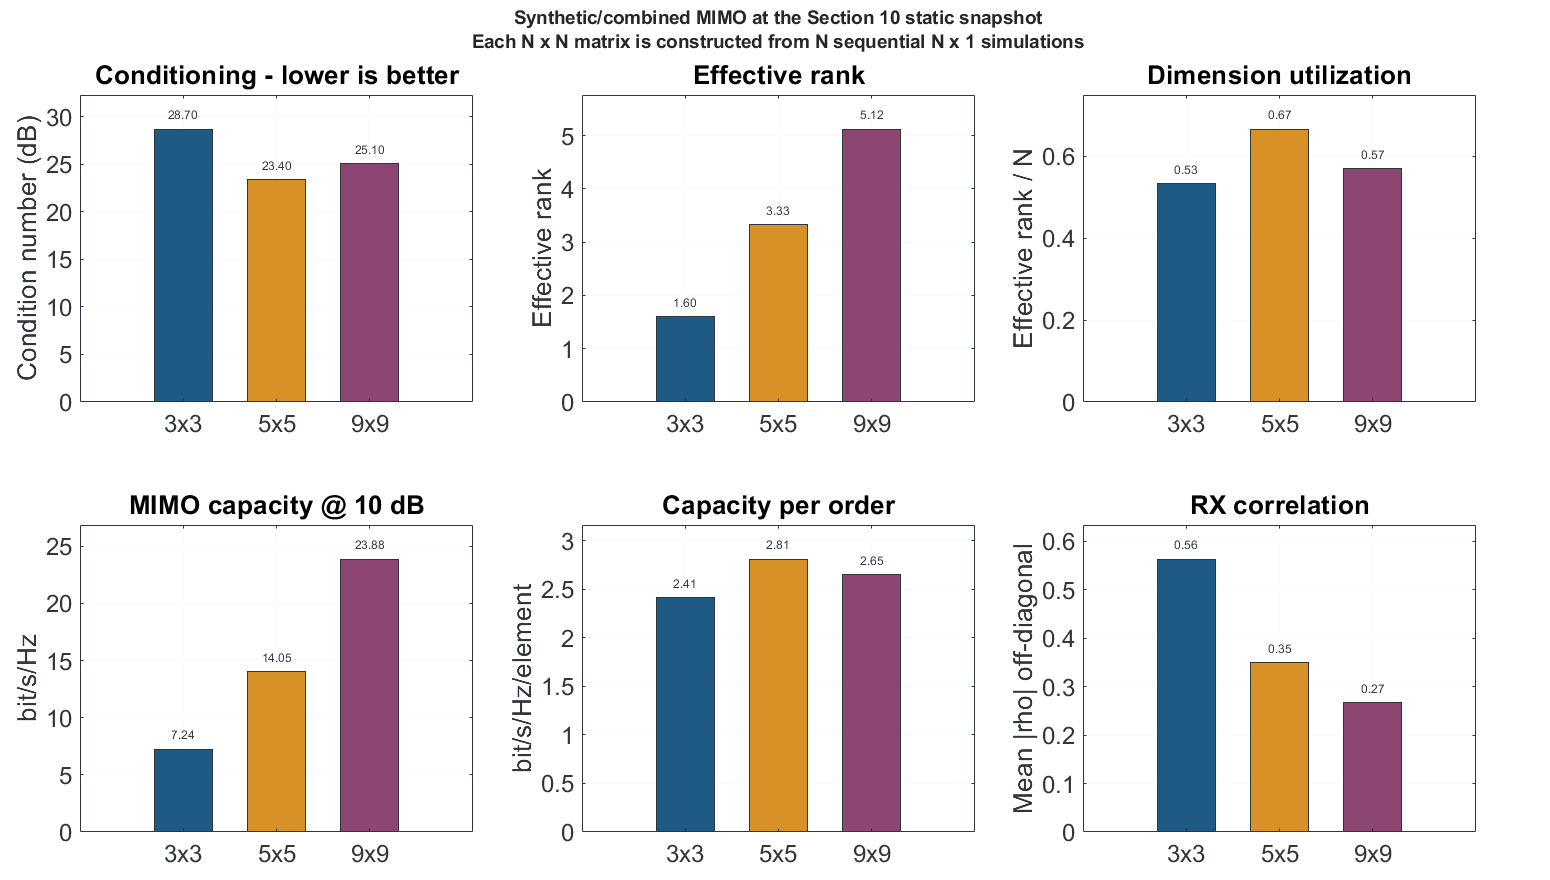
\includegraphics[width=0.98\linewidth]{Images/Analisis_v4_ISO_TX_Lens_Order_3x3_5x5_9x9_Linear/figures_matlab/03_static_mimo_scaling_matlab.png}
    \caption{Constructed static $N\times N$ MIMO metrics versus order. The $5\times5$ configuration is best conditioned and has the highest effective-rank fraction and capacity per dimension in this single snapshot.}
    \label{fig:iso-order-static-mimo}
\end{figure}

\subsection{Aggregate and Along-Trajectory Link Scaling}

Table~\ref{tab:iso-order-aggregate-results} and Figure~\ref{fig:iso-order-aggregate} summarize the trajectory results. The median channel magnitude varies by only 0.29~dB across the three orders, whereas the median link capacity rises from 3.57 to 5.19~bit/s/Hz. The 1.62~bit/s/Hz increase from $N=3$ to $N=9$ corresponds to 45.4\%, but it occurs together with a 4.77~dB increase in nominal total TX power. Outage at the 1~bit/s/Hz threshold is 0\% for every order and is therefore non-discriminating.

\begin{table}[htbp]
    \centering
    \caption{Aggregate link, constructed-MIMO, and spatial-decorrelation metrics along the common linear trajectory. The channel-magnitude summary uses all 16 mobility samples, whereas the link and constructed-MIMO metrics use the first sample at each waypoint. The two capacity metrics are in bit/s/Hz; $D_\mathrm{global}$ and $D_\mathrm{med}$ denote global-pooled and block-median decorrelation, respectively, computed from all 16 samples.}
    \label{tab:iso-order-aggregate-results}
    \footnotesize
    \renewcommand{\arraystretch}{1.13}
    \begin{tabularx}{\linewidth}{@{}>{\raggedright\arraybackslash}X *{3}{>{\centering\arraybackslash}p{0.145\linewidth}}@{}}
        \toprule
        \textbf{Metric} & \textbf{$3\times3$} & \textbf{$5\times5$} & \textbf{$9\times9$} \\
        \midrule
        Nominal total TX power (dBm) & 14.77 & 16.99 & 19.54 \\
        Median channel magnitude (dB) & $-86.75$ & $-86.94$ & $-86.65$ \\
        Median link capacity & 3.57 & 4.13 & 5.19 \\
        Median condition number (dB) & 25.55 & 34.24 & 42.88 \\
        Median effective rank & 1.154 & 1.332 & 2.043 \\
        Effective rank fraction, $\eta_r$ & 0.385 & 0.266 & 0.227 \\
        Median MIMO capacity at 10~dB & 5.851 & 8.254 & 14.562 \\
        MIMO capacity per dimension, $\eta_C$ & 1.950 & 1.651 & 1.618 \\
        $D_\mathrm{global}$ & 0.9807 & 0.9276 & 0.8570 \\
        $D_\mathrm{med}$ & 0.5308 & 0.5166 & 0.4876 \\
        \bottomrule
    \end{tabularx}
\end{table}

\clearpage
\begin{figure}[p]
    \centering
    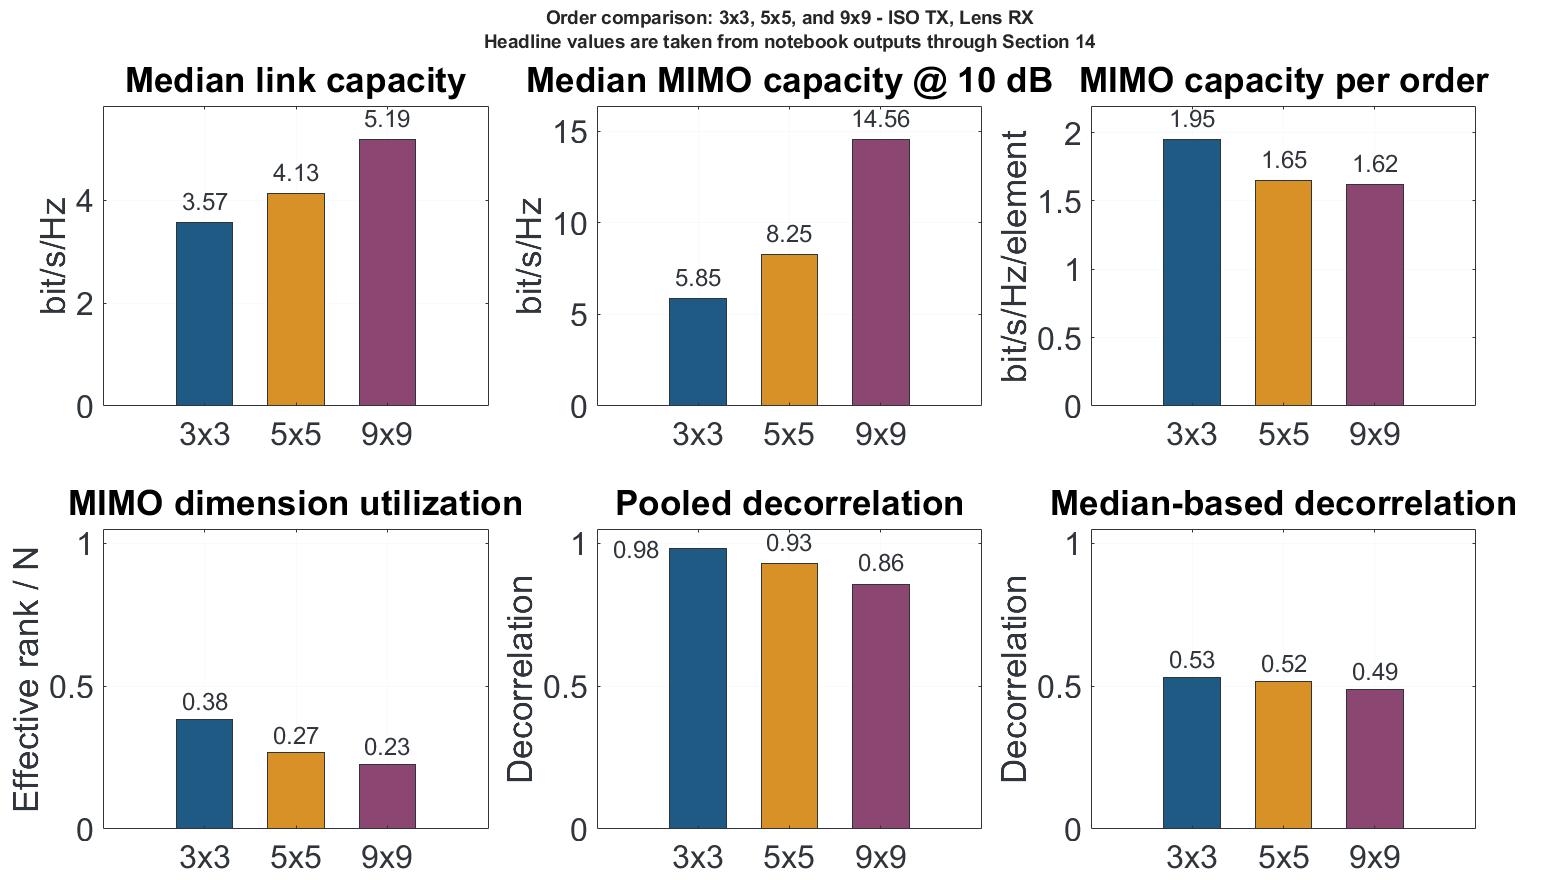
\includegraphics[width=\linewidth]{Images/Analisis_v4_ISO_TX_Lens_Order_3x3_5x5_9x9_Linear/figures_matlab/08_aggregate_order_comparison_matlab.png}
    \caption{Aggregate link, constructed-MIMO, dimension-normalized, and spatial-decorrelation metrics for the three lens-assisted orders along the common linear trajectory.}
    \label{fig:iso-order-aggregate}
\end{figure}
\clearpage

The common $0^\circ$ RX branch reduces the confounding effect of the changing angular populations, although it does not remove the differences in nominal total TX power and aperture. Its median channel magnitude changes from $-86.85$ to $-87.41$~dB between $N=3$ and $N=9$, while the SNR rises from 10.70 to 14.96~dB and the link capacity increases from 3.54 to 4.96~bit/s/Hz. The combination of a slightly weaker channel response and a higher SNR is consistent with the increase in nominal total TX power; it does not demonstrate a power-independent order gain.

Figure~\ref{fig:iso-order-link-trajectory} shows the mean channel magnitude and link capacity at each waypoint. The shaded regions are the minimum-to-maximum ranges across the RX branches at a given order, not confidence intervals. Capacity generally rises with order, but the changing band widths and local crossings show that the benefit depends on position and lens angle.

\begin{figure}[htbp]
    \centering
    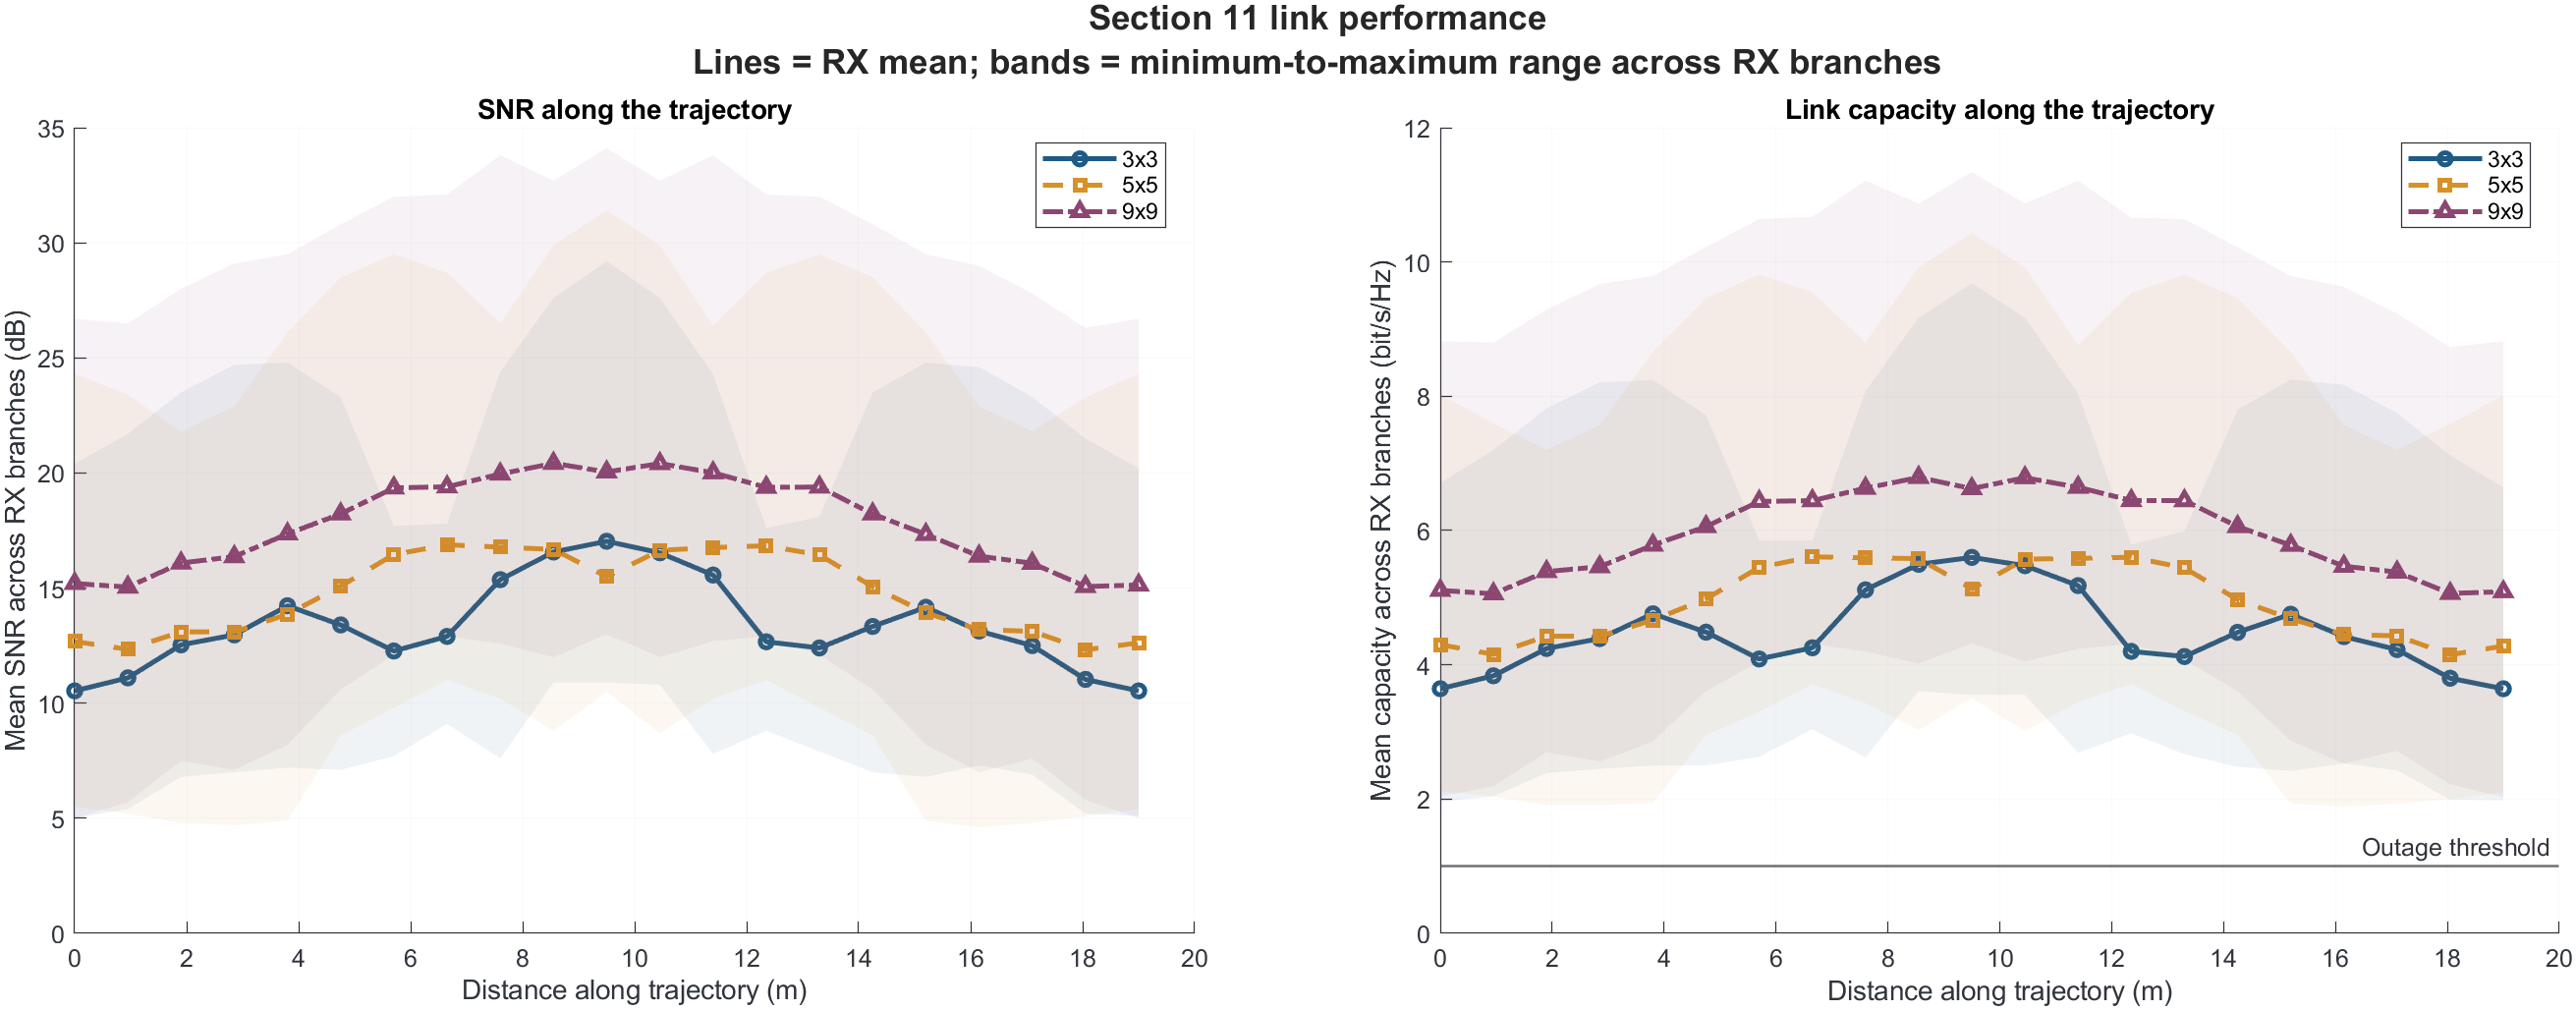
\includegraphics[width=\linewidth]{Images/Analisis_v4_ISO_TX_Lens_Order_3x3_5x5_9x9_Linear/figures_matlab/04_channel_along_trajectory_matlab.png}
    \caption{Mean channel magnitude and link-budget capacity along the common linear trajectory. Channel magnitude uses all 16 mobility samples, whereas capacity uses the first sample at each waypoint. Shaded regions indicate the minimum-to-maximum range across RX lens branches, not statistical confidence intervals.}
    \label{fig:iso-order-link-trajectory}
\end{figure}

\subsection{Constructed MIMO Scaling Along the Trajectory}

The constructed MIMO capacity increases from 5.851 to 14.562~bit/s/Hz between $N=3$ and $N=9$, an increase of 8.711~bit/s/Hz, or approximately 148.9\%. The absolute effective rank also rises from 1.154 to 2.043. These gains are nevertheless sublinear in the number of dimensions. Over the same comparison, the effective-rank fraction decreases from 0.385 to 0.227, a relative reduction of approximately 41.0\%, and the capacity per dimension decreases from 1.950 to 1.618~bit/s/Hz, or approximately 17.0\%. Concurrently, the median condition number worsens by 17.33~dB, from 25.55 to 42.88~dB. Higher order therefore adds normalized constructed capacity, but the additional dimensions are progressively less balanced and less efficiently utilized.

Figure~\ref{fig:iso-order-mimo-trajectory} also shows a shared bottleneck at the 9.5~m trajectory midpoint. The condition number reaches 55.09, 62.06, and 71.89~dB for $N=3$, $5$, and $9$, respectively; the effective rank falls to 1.035, 1.061, and 1.085; and the MIMO capacities reach their respective trajectory minima of 5.185, 6.251, and 7.842~bit/s/Hz. The occurrence of this impairment at the same waypoint for all orders indicates sensitivity to the common path geometry. It also explains why the nonmonotonic static ordering does not persist in the trajectory medians.

\clearpage
\begin{figure}[p]
    \centering
    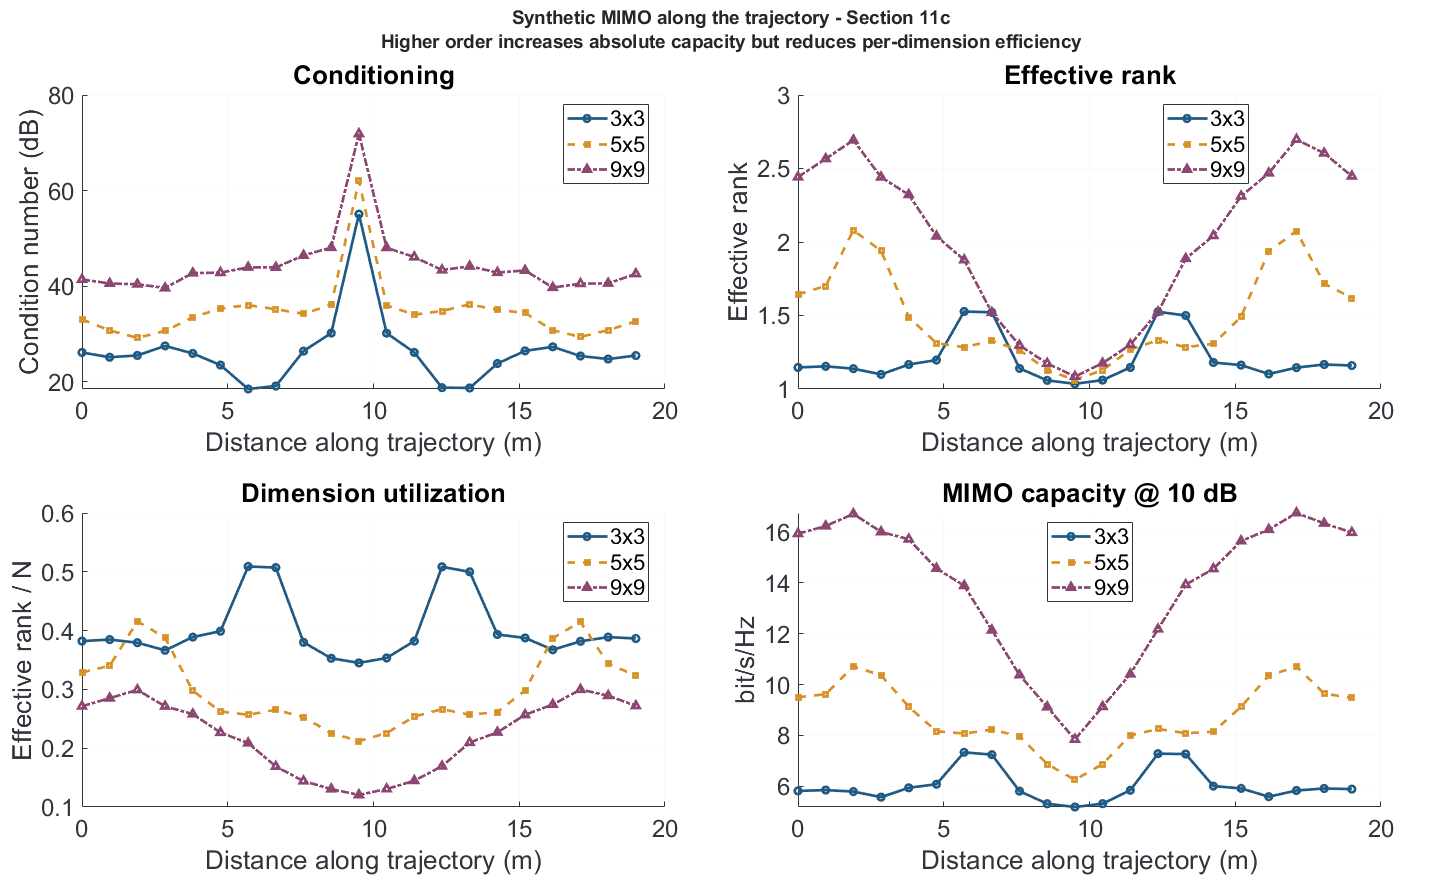
\includegraphics[width=\linewidth]{Images/Analisis_v4_ISO_TX_Lens_Order_3x3_5x5_9x9_Linear/figures_matlab/05_trajectory_mimo_scaling_matlab.png}
    \caption{Condition number, effective rank, effective-rank fraction, and ideal normalized MIMO capacity at 10~dB for the constructed $N\times N$ channels along the common trajectory. All orders exhibit a midpoint bottleneck.}
    \label{fig:iso-order-mimo-trajectory}
\end{figure}
\clearpage

\subsection{Spatial Decorrelation Across Orders}

Both aggregate decorrelation estimators decrease monotonically with order. Global-pooled decorrelation falls from 0.9807 for $N=3$ to 0.9276 for $N=5$ and 0.8570 for $N=9$. The block-median estimator decreases more modestly, from 0.5308 to 0.5166 and 0.4876. This indicates greater average similarity among the center-TX RX responses in the higher-order configurations under the respective aggregation rules. It does not establish an order-only effect because the number of RX pairs increases from 3 to 10 to 36, and the $9\times9$ grid introduces many closely spaced $15^\circ$ pairs. The number and spacing of RX lens angles therefore change together with $N$.

Figure~\ref{fig:iso-order-decorrelation} presents waypoint-local rather than global-pooled estimates. The mean waypoint-local pooled values are 0.5502, 0.5215, and 0.4934, while the corresponding mean median-based values are 0.5414, 0.5110, and 0.4836. Their overall ordering agrees with the aggregate summary, but the curves cross along the path. Hence, $N=3$ is not more decorrelated at every waypoint, and numerical values from the local curves should not be substituted for the global statistics in Table~\ref{tab:iso-order-aggregate-results}.

\begin{figure}[htbp]
    \centering
    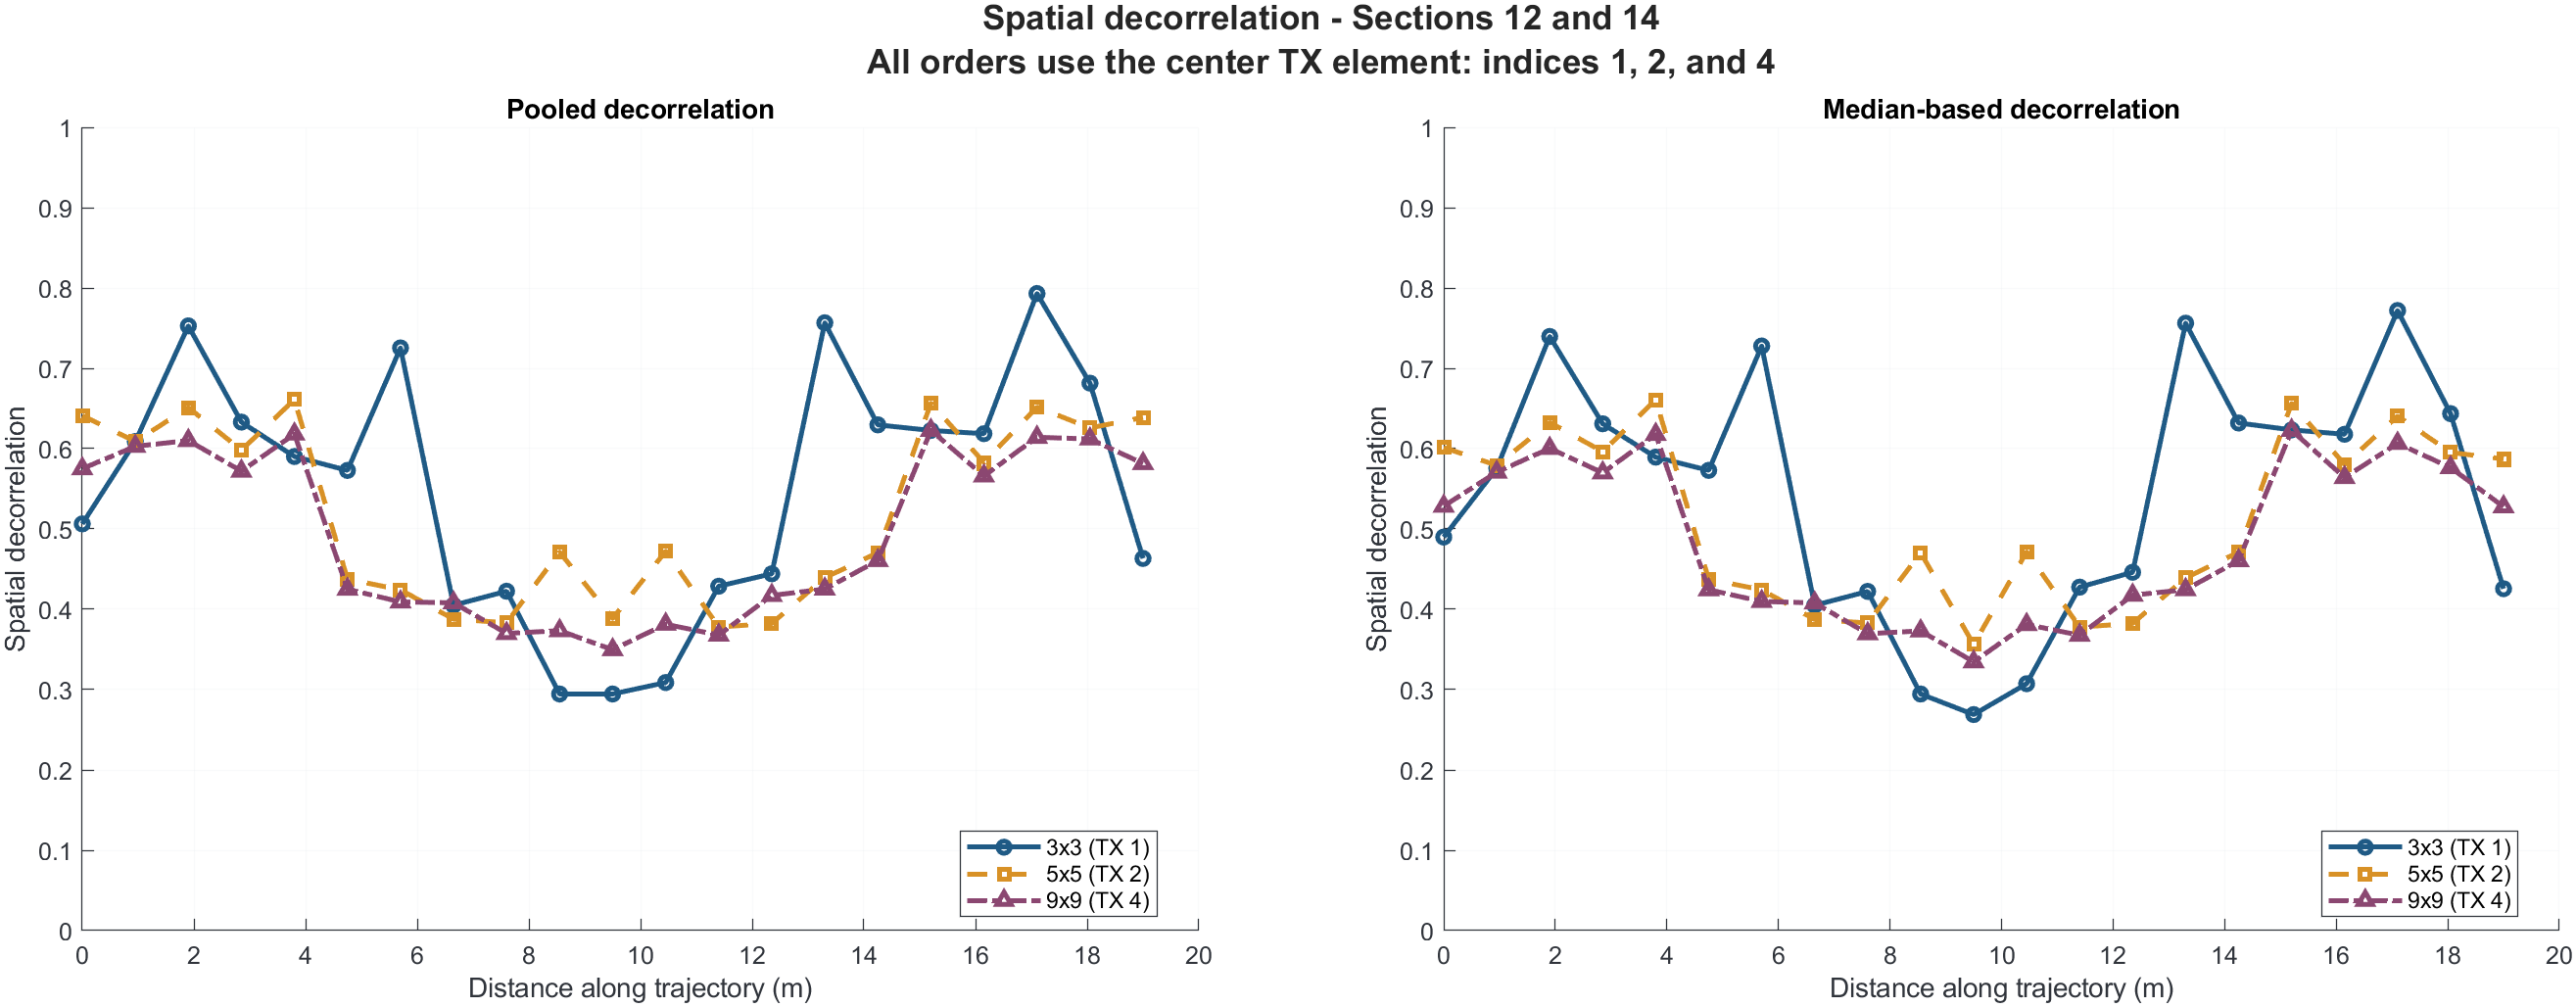
\includegraphics[width=\linewidth]{Images/Analisis_v4_ISO_TX_Lens_Order_3x3_5x5_9x9_Linear/figures_matlab/06_spatial_decorrelation_by_order_matlab.png}
    \caption{Waypoint-local pooled and median-based decorrelation of the center-TX responses across RX lens branches, using all 16 mobility samples. The curves cross locally even though their trajectory averages decrease with order.}
    \label{fig:iso-order-decorrelation}
\end{figure}

The mean raw difference power in Figure~\ref{fig:iso-order-raw-difference} is nonmonotonic: $4.863\times10^{-8}$, $4.205\times10^{-8}$, and $4.628\times10^{-8}$ for $N=3$, $5$, and $9$, respectively. Because this metric preserves path loss and pattern gain, it neither contradicts the normalized decorrelation result nor serves as an independent measure of spatial-channel quality.

\begin{figure}[htbp]
    \centering
    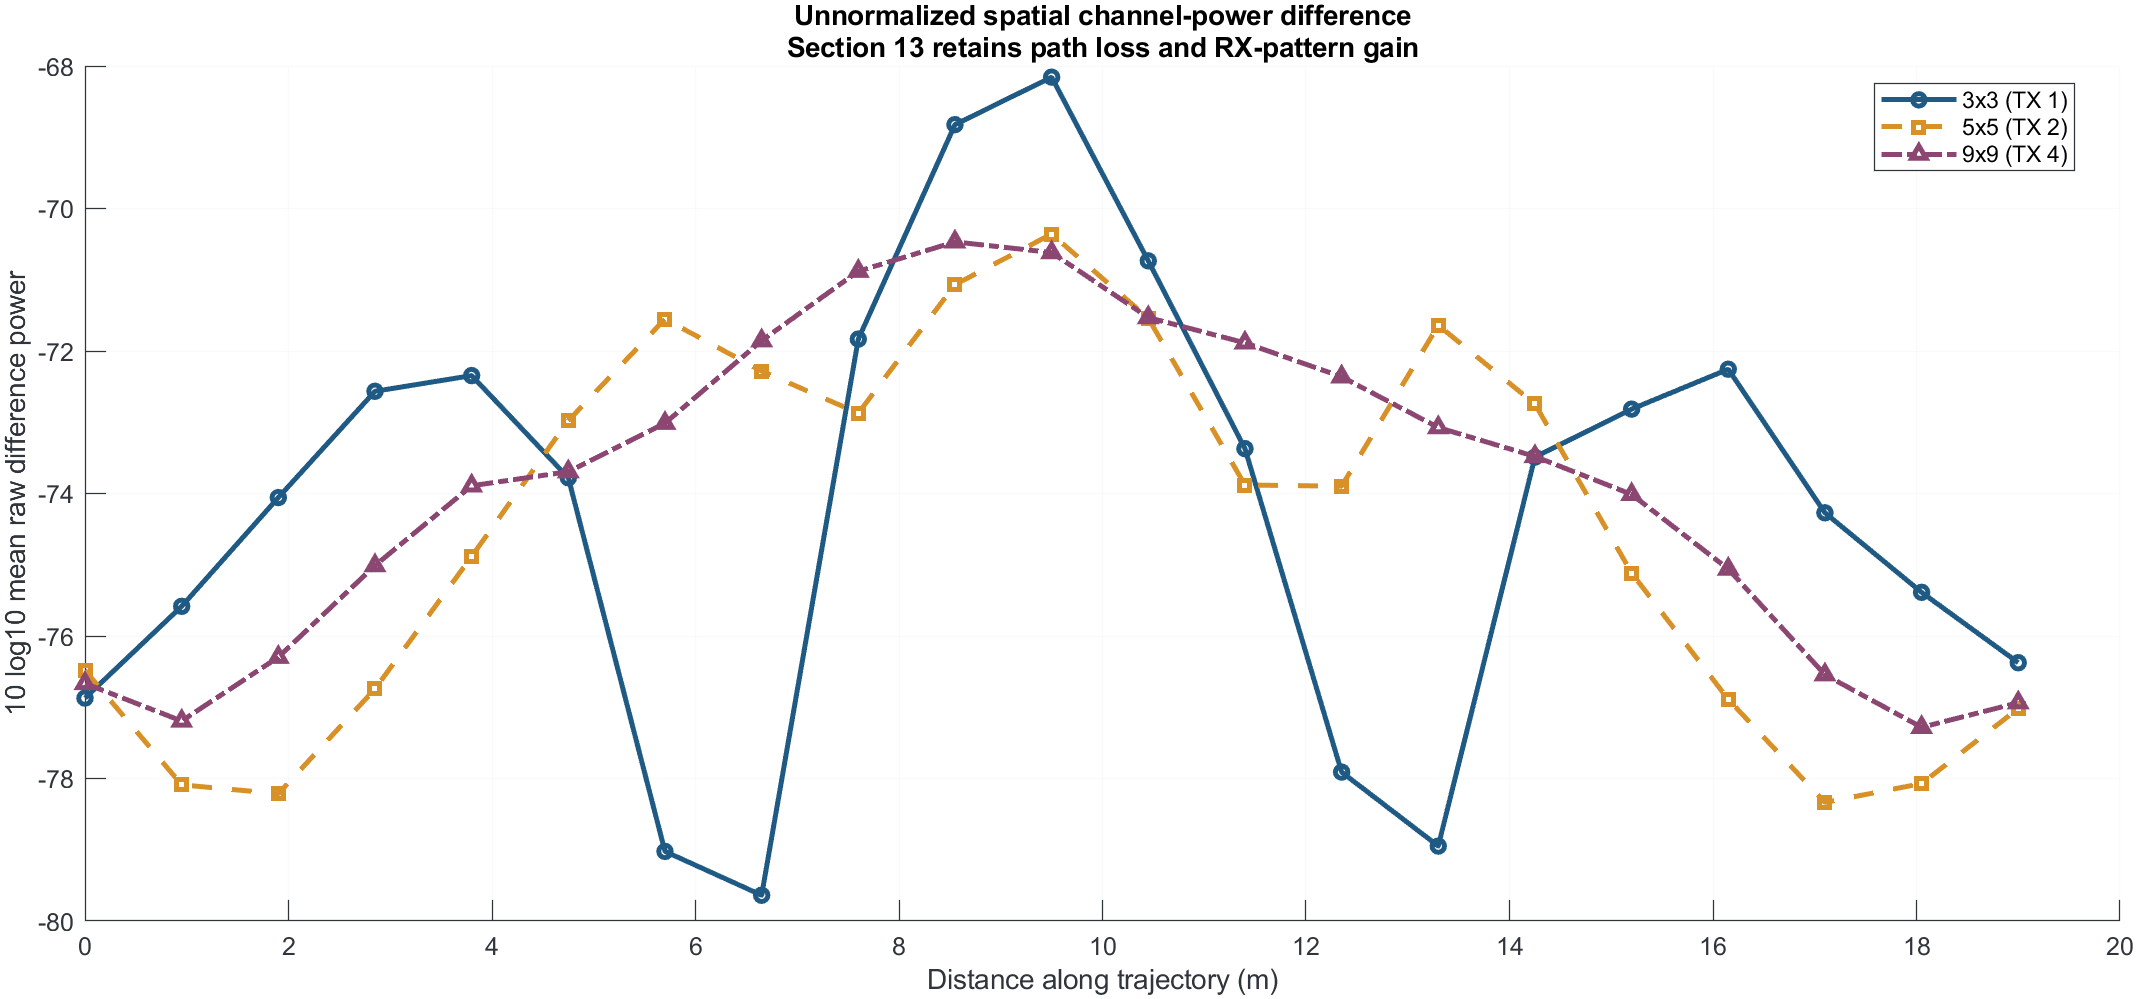
\includegraphics[width=0.95\linewidth]{Images/Analisis_v4_ISO_TX_Lens_Order_3x3_5x5_9x9_Linear/figures_matlab/07_raw_spatial_difference_by_order_matlab.png}
    \caption{Raw center-TX spatial difference power across RX lens branches. The metric is amplitude-sensitive and shows no monotonic order trend.}
    \label{fig:iso-order-raw-difference}
\end{figure}

\subsection{Discussion and Limitations}

The higher-order comparison shows that aggregate capacity and normalized spatial efficiency answer different design questions. In the link budget, activating more TX elements increases the nominal total TX power and the reported capacity. Separately, the larger constructed matrix supports a higher normalized MIMO capacity at the same 10~dB reference SNR. However, the rise in effective rank is much smaller than the rise in $N$, the singular-value spread grows, and both normalized metrics in Equation~\ref{eq:iso-order-normalized-metrics} decrease. Under the evaluated configurations, higher order therefore offers additional constructed capacity with diminishing utilization of each added spatial dimension.

Position sensitivity is also important. At the static snapshot, $N=5$ has the best condition number and normalized efficiencies, whereas the full-trajectory condition number and normalized efficiencies worsen monotonically with $N$. All three configurations experience their worst conditioning and minimum MIMO capacity at the same path midpoint. A single static position can therefore overstate or reverse the order ranking, and higher-order design should be evaluated over its intended motion and orientation distribution.

Several factors prevent causal attribution to $N$ alone. First, 10~dBm is assigned to every TX, so nominal total TX power increases from 14.77 to 19.54~dBm. Second, fixed 0.45~m spacing causes a fourfold aperture increase, and the RX angle grids change in both extent and resolution. Third, only the $0^\circ$ RX branch is common across all orders. Controlled follow-up studies should separately hold nominal total TX power, aperture, and RX angles constant to quantify their individual contributions.

The channel construction imposes further limitations. Each $N\times N$ matrix stacks $N$ sequential $N\times1$ simulations rather than simultaneous multiport RX measurements; mutual coupling, a common receiver hardware phase reference, joint combining, and switching overhead are not represented. The link-budget and constructed-MIMO metrics also use only the first of the 16 mobility time samples at each waypoint, so their trajectory variation describes changes between waypoints rather than the within-waypoint Doppler distribution. The results cover one room and one trajectory without a multi-seed convergence study or confidence intervals. The ray-tracing run uses 100{,}000 path samples per source rather than the 1{,}000{,}000 recommended by the source workflow for a final high-accuracy run. The 1~bit/s/Hz outage threshold is saturated, and the fixed-SNR MIMO capacity is an ideal channel-structure metric rather than coded throughput. Finally, the source notebooks and the derived CSV tables and figures are present, and the latter pass all 21 packaged validation checks; however, the complete complex CFR tensors are not exported as separate archival data. Alternative channel-level analyses therefore require rerunning the source notebooks rather than operating directly on a retained CFR tensor.

\subsection{Summary of Higher-Order Scaling}

Along the common lens-assisted linear trajectory, scaling from $3\times3$ to $9\times9$ increases median link capacity from 3.57 to 5.19~bit/s/Hz and constructed-MIMO capacity at 10~dB from 5.851 to 14.562~bit/s/Hz. The gain is not proportional: median condition number worsens by 17.33~dB, effective-rank fraction falls from 0.385 to 0.227, capacity per dimension falls from 1.950 to 1.618~bit/s/Hz, and both aggregate decorrelation estimators decrease. Higher order therefore increases both link capacity and normalized constructed-MIMO capacity with diminishing spatial efficiency, but the present results do not establish a fixed-total-power or fixed-aperture advantage.
